%% 由 build/emit_tex.py 生成（生成物，勿手改）；定制请放 user_style.tex / user_meta.yaml
\chapter{Numpy及其基本使用}\label{numpyux53caux5176ux57faux672cux4f7fux7528}

\section{01
数组基础：创建、属性、索引、广播与随机数}\label{ux6570ux7ec4ux57faux7840ux521bux5efaux5c5eux6027ux7d22ux5f15ux5e7fux64adux4e0eux968fux673aux6570}

\begin{quote}
本节对应原版 1.1 的内容，并增补学习目标、常见误区、思考题与延伸阅读。
配套图：\texttt{figures/01-numpy/reshape.png}、\texttt{figures/01-numpy/broadcast.png}（由
\texttt{build/make\_chap1\_figures.py} 生成）。
\end{quote}

\subsection{本节目标}\label{ux672cux8282ux76eeux6807}

\begin{itemize}
\tightlist
\item
  理解 \texttt{ndarray} 是什么，以及它与 Python 列表的区别；
\item
  会创建常见数组（\texttt{array}、\texttt{zeros}、\texttt{ones}、\texttt{full}、\texttt{arange}、\texttt{linspace}、\texttt{diag}、\texttt{eye}）；
\item
  掌握
  \texttt{shape}、\texttt{ndim}、\texttt{dtype}、\texttt{size}、\texttt{itemsize}
  等属性；
\item
  掌握索引、切片、花式索引、布尔掩码；
\item
  理解\textbf{视图（view）与拷贝（copy）}，知道 \texttt{reshape}
  \texttt{ravel} \texttt{flatten} \texttt{copy} 的区别；
\item
  掌握广播规则，能手工判断形状是否兼容；
\item
  使用新版随机数生成器
  \texttt{Generator}（\texttt{default\_rng}）生成可复现随机数。
\end{itemize}

\subsection{先修}\label{ux5148ux4fee}

\begin{itemize}
\tightlist
\item
  Python 列表、元组、循环、函数；了解变量类型的含义。
\end{itemize}

\begin{center}\rule{0.5\linewidth}{0.5pt}\end{center}

\subsection{1.1 为什么用 NumPy}\label{ux4e3aux4ec0ux4e48ux7528-numpy}

Python 列表方便但``慢''，且不能直接做向量化运算。NumPy 的
\texttt{ndarray} 由 C
实现，元素类型统一，支持逐元素运算与广播，这正是科学计算需要的能力。

{\def\LTcaptype{none} % do not increment counter
\begin{longtable}[]{@{}lll@{}}
\toprule\noalign{}
特性 & Python list & NumPy ndarray \\
\midrule\noalign{}
\endhead
\bottomrule\noalign{}
\endlastfoot
元素类型 & 可混合 & 必须统一（dtype） \\
逐元素运算 & 需循环/列表推导 & 直接 \texttt{a\ +\ b} \\
内存 & 对象指针数组 & 连续内存块 \\
速度 & 慢 & 快（向量化） \\
\end{longtable}
}

\subsection{1.2 创建数组}\label{ux521bux5efaux6570ux7ec4}

\subsubsection{1.2.1
从列表/元组创建}\label{ux4eceux5217ux8868ux5143ux7ec4ux521bux5efa}

\begin{Shaded}
\begin{Highlighting}[]
\ImportTok{import}\NormalTok{ numpy }\ImportTok{as}\NormalTok{ np}

\NormalTok{x }\OperatorTok{=}\NormalTok{ np.array([}\DecValTok{1}\NormalTok{, }\DecValTok{2}\NormalTok{, }\DecValTok{3}\NormalTok{, }\DecValTok{4}\NormalTok{, }\DecValTok{5}\NormalTok{])        }\CommentTok{\# 一维数组}
\NormalTok{y }\OperatorTok{=}\NormalTok{ np.array([[}\DecValTok{1}\NormalTok{, }\DecValTok{2}\NormalTok{, }\DecValTok{3}\NormalTok{], [}\DecValTok{4}\NormalTok{, }\DecValTok{5}\NormalTok{, }\DecValTok{6}\NormalTok{]]) }\CommentTok{\# 二维数组（矩阵）}
\BuiltInTok{print}\NormalTok{(x, x.shape, x.dtype)}
\BuiltInTok{print}\NormalTok{(y, y.shape, y.ndim)}
\BuiltInTok{print}\NormalTok{(}\BuiltInTok{type}\NormalTok{(x))}
\end{Highlighting}
\end{Shaded}

\begin{Shaded}
\begin{Highlighting}[]
\NormalTok{[1 2 3 4 5] (5,) int64}
\NormalTok{[[1 2 3]}
\NormalTok{ [4 5 6]] (2, 3) 2}
\NormalTok{\textless{}class \textquotesingle{}numpy.ndarray\textquotesingle{}\textgreater{}}
\end{Highlighting}
\end{Shaded}

\begin{quote}
\textbf{注意}：子数组长度必须一致；\texttt{np.array({[}{[}1,2{]},{[}3{]}{]})}
会报错或产生 object 数组。
\end{quote}

\subsubsection{1.2.2
指定数据类型}\label{ux6307ux5b9aux6570ux636eux7c7bux578b}

\begin{Shaded}
\begin{Highlighting}[]
\NormalTok{x }\OperatorTok{=}\NormalTok{ np.array([}\DecValTok{1}\NormalTok{, }\DecValTok{2}\NormalTok{, }\DecValTok{3}\NormalTok{], dtype}\OperatorTok{=}\NormalTok{np.int32)}
\BuiltInTok{print}\NormalTok{(x.dtype, x.itemsize)   }\CommentTok{\# int32 4}

\NormalTok{x2 }\OperatorTok{=}\NormalTok{ x.astype(np.float64)}
\BuiltInTok{print}\NormalTok{(x2.dtype, x2.itemsize) }\CommentTok{\# float64 8}

\CommentTok{\#\# 与 Python 列表互转}
\NormalTok{lst }\OperatorTok{=}\NormalTok{ x.tolist()      }\CommentTok{\# 或 list(x)}
\NormalTok{arr }\OperatorTok{=}\NormalTok{ np.array(lst)}
\end{Highlighting}
\end{Shaded}

\textbf{内存开销}：\texttt{astype}
默认返回新数组（拷贝）；如仅查看数值但不改，可避免不必要的转换。

\subsubsection{1.2.3 快速创建}\label{ux5febux901fux521bux5efa}

\begin{Shaded}
\begin{Highlighting}[]
\NormalTok{np.zeros((}\DecValTok{2}\NormalTok{, }\DecValTok{3}\NormalTok{))            }\CommentTok{\# 全 0，形状 (2,3)}
\NormalTok{np.ones((}\DecValTok{2}\NormalTok{, }\DecValTok{3}\NormalTok{))             }\CommentTok{\# 全 1}
\NormalTok{np.full((}\DecValTok{2}\NormalTok{, }\DecValTok{3}\NormalTok{), }\DecValTok{42}\NormalTok{)         }\CommentTok{\# 全 42}
\NormalTok{np.arange(}\DecValTok{0}\NormalTok{, }\DecValTok{11}\NormalTok{, }\DecValTok{2}\NormalTok{)         }\CommentTok{\# [ 0  2  4  6  8 10]}
\NormalTok{np.linspace(}\DecValTok{0}\NormalTok{, }\DecValTok{10}\NormalTok{, }\DecValTok{5}\NormalTok{)       }\CommentTok{\# [ 0.  2.5  5.  7.5 10. ]}
\NormalTok{np.diag([}\DecValTok{1}\NormalTok{, }\DecValTok{2}\NormalTok{, }\DecValTok{3}\NormalTok{])          }\CommentTok{\# 对角线矩阵}
\NormalTok{np.eye(}\DecValTok{3}\NormalTok{)                   }\CommentTok{\# 3x3 单位矩阵}
\NormalTok{np.eye(}\DecValTok{3}\NormalTok{, }\DecValTok{4}\NormalTok{)                }\CommentTok{\# 3x4，主对角线为 1}
\NormalTok{np.eye(}\DecValTok{3}\NormalTok{, k}\OperatorTok{=}\DecValTok{1}\NormalTok{)              }\CommentTok{\# 主对角线上方一条对角线为 1}
\end{Highlighting}
\end{Shaded}

\begin{Shaded}
\begin{Highlighting}[]
\BuiltInTok{print}\NormalTok{(np.arange(}\DecValTok{5}\NormalTok{))          }\CommentTok{\# [0 1 2 3 4]}
\BuiltInTok{print}\NormalTok{(np.linspace(}\DecValTok{0}\NormalTok{, }\DecValTok{1}\NormalTok{, }\DecValTok{3}\NormalTok{))  }\CommentTok{\# [0.  0.5 1. ]}
\BuiltInTok{print}\NormalTok{(np.diag([}\DecValTok{1}\NormalTok{, }\DecValTok{2}\NormalTok{, }\DecValTok{3}\NormalTok{]))}
\end{Highlighting}
\end{Shaded}

\begin{Shaded}
\begin{Highlighting}[]
\NormalTok{[0 1 2 3 4]}
\NormalTok{[0.  0.5 1. ]}
\NormalTok{[[1 0 0]}
\NormalTok{ [0 2 0]}
\NormalTok{ [0 0 3]]}
\end{Highlighting}
\end{Shaded}

\begin{quote}
提醒：\texttt{zeros}/\texttt{ones}/\texttt{full}
的形状参数是\textbf{元组}（两个括号）；\texttt{arange} 类似
\texttt{range}，终点是开区间。
\end{quote}

\subsubsection{1.2.4 数组属性}\label{ux6570ux7ec4ux5c5eux6027}

\begin{Shaded}
\begin{Highlighting}[]
\NormalTok{a }\OperatorTok{=}\NormalTok{ np.arange(}\DecValTok{24}\NormalTok{).reshape(}\DecValTok{2}\NormalTok{, }\DecValTok{3}\NormalTok{, }\DecValTok{4}\NormalTok{)}
\BuiltInTok{print}\NormalTok{(}\StringTok{"shape:"}\NormalTok{, a.shape)   }\CommentTok{\# 各维长度}
\BuiltInTok{print}\NormalTok{(}\StringTok{"ndim :"}\NormalTok{, a.ndim)    }\CommentTok{\# 维数 3}
\BuiltInTok{print}\NormalTok{(}\StringTok{"size :"}\NormalTok{, a.size)    }\CommentTok{\# 元素总数 24}
\BuiltInTok{print}\NormalTok{(}\StringTok{"dtype:"}\NormalTok{, a.dtype)   }\CommentTok{\# 数据类型}
\BuiltInTok{print}\NormalTok{(}\StringTok{"itemsize:"}\NormalTok{, a.itemsize)  }\CommentTok{\# 单元素字节数}
\end{Highlighting}
\end{Shaded}

\begin{center}\rule{0.5\linewidth}{0.5pt}\end{center}

\subsection{1.3
变形、转置与拼接}\label{ux53d8ux5f62ux8f6cux7f6eux4e0eux62fcux63a5}

\subsubsection{1.3.1 reshape}\label{reshape}

\begin{Shaded}
\begin{Highlighting}[]
\NormalTok{arr }\OperatorTok{=}\NormalTok{ np.arange(}\DecValTok{6}\NormalTok{)}
\BuiltInTok{print}\NormalTok{(arr.reshape((}\DecValTok{2}\NormalTok{, }\DecValTok{3}\NormalTok{)))   }\CommentTok{\# 或 arr.reshape(2, 3)}
\BuiltInTok{print}\NormalTok{(arr.reshape((}\DecValTok{3}\NormalTok{, }\OperatorTok{{-}}\DecValTok{1}\NormalTok{)))  }\CommentTok{\# {-}1 自动推断：3×2}
\BuiltInTok{print}\NormalTok{(arr.reshape(}\OperatorTok{{-}}\DecValTok{1}\NormalTok{))       }\CommentTok{\# 展平为一维}
\end{Highlighting}
\end{Shaded}

\begin{figure}
\centering
\pandocbounded{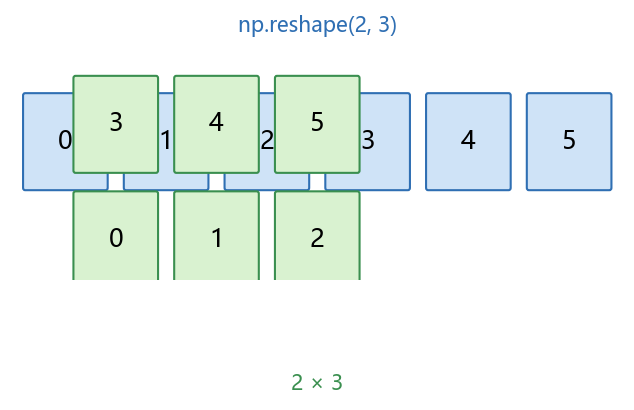
\includegraphics[keepaspectratio,alt={reshape 示意图}]{figures/01-numpy/reshape.png}}
\caption{reshape 示意图}
\end{figure}

\begin{itemize}
\tightlist
\item
  总元素数必须相等；
\item
  \texttt{reshape}
  在内存连续时通常返回\textbf{视图}（共享内存）；需要独立副本时用
  \texttt{arr.reshape(...).copy()}。
\end{itemize}

\subsubsection{1.3.2 展平：ravel vs
flatten}\label{ux5c55ux5e73ravel-vs-flatten}

\begin{Shaded}
\begin{Highlighting}[]
\NormalTok{a }\OperatorTok{=}\NormalTok{ np.array([[}\DecValTok{1}\NormalTok{, }\DecValTok{2}\NormalTok{, }\DecValTok{3}\NormalTok{], [}\DecValTok{4}\NormalTok{, }\DecValTok{5}\NormalTok{, }\DecValTok{6}\NormalTok{]])}
\NormalTok{a.ravel()    }\CommentTok{\# 视图（尽可能不拷贝）}
\NormalTok{a.flatten()  }\CommentTok{\# 总是拷贝}
\NormalTok{a.reshape(}\OperatorTok{{-}}\DecValTok{1}\NormalTok{)  }\CommentTok{\# 展平}
\end{Highlighting}
\end{Shaded}

\subsubsection{1.3.3 转置}\label{ux8f6cux7f6e}

\begin{Shaded}
\begin{Highlighting}[]
\NormalTok{a }\OperatorTok{=}\NormalTok{ np.arange(}\DecValTok{6}\NormalTok{).reshape(}\DecValTok{2}\NormalTok{, }\DecValTok{3}\NormalTok{)}
\NormalTok{a.T          }\CommentTok{\# 转置 (3,2)}
\NormalTok{np.transpose(a)            }\CommentTok{\# 等价}
\NormalTok{np.transpose(a, axes}\OperatorTok{=}\NormalTok{(}\DecValTok{1}\NormalTok{, }\DecValTok{0}\NormalTok{))  }\CommentTok{\# 高维时可指定轴的顺序}
\end{Highlighting}
\end{Shaded}

\subsubsection{1.3.4 拼接与堆叠}\label{ux62fcux63a5ux4e0eux5806ux53e0}

\begin{Shaded}
\begin{Highlighting}[]
\NormalTok{a }\OperatorTok{=}\NormalTok{ np.array([[}\DecValTok{1}\NormalTok{, }\DecValTok{2}\NormalTok{], [}\DecValTok{3}\NormalTok{, }\DecValTok{4}\NormalTok{]])}
\NormalTok{b }\OperatorTok{=}\NormalTok{ np.array([[}\DecValTok{5}\NormalTok{, }\DecValTok{6}\NormalTok{]])}
\NormalTok{np.concatenate((a, b), axis}\OperatorTok{=}\DecValTok{0}\NormalTok{)      }\CommentTok{\# 沿 0 轴拼接: (3,2)}
\NormalTok{np.concatenate((a, a), axis}\OperatorTok{=}\DecValTok{1}\NormalTok{)      }\CommentTok{\# 沿 1 轴拼接: (2,4)}
\NormalTok{np.vstack((a, b))                   }\CommentTok{\# 垂直堆叠}
\NormalTok{np.hstack((a, a))                   }\CommentTok{\# 水平堆叠}
\NormalTok{np.stack(([}\DecValTok{1}\NormalTok{, }\DecValTok{2}\NormalTok{], [}\DecValTok{3}\NormalTok{, }\DecValTok{4}\NormalTok{]), axis}\OperatorTok{=}\DecValTok{0}\NormalTok{)  }\CommentTok{\# 新增维度堆叠 (2,2)}
\NormalTok{np.column\_stack(([}\DecValTok{1}\NormalTok{, }\DecValTok{2}\NormalTok{], [}\DecValTok{3}\NormalTok{, }\DecValTok{4}\NormalTok{]))   }\CommentTok{\# 一维数组按列堆叠 (2,2)}
\end{Highlighting}
\end{Shaded}

\subsubsection{1.3.5 增删元素}\label{ux589eux5220ux5143ux7d20}

\begin{Shaded}
\begin{Highlighting}[]
\NormalTok{a }\OperatorTok{=}\NormalTok{ np.array([}\DecValTok{1}\NormalTok{, }\DecValTok{2}\NormalTok{, }\DecValTok{3}\NormalTok{])}
\NormalTok{np.append(a, }\DecValTok{4}\NormalTok{)              }\CommentTok{\# 返回新数组 [1 2 3 4]}
\NormalTok{np.delete(a, }\DecValTok{1}\NormalTok{)              }\CommentTok{\# 返回新数组 [1 3]}
\NormalTok{a[[}\DecValTok{0}\NormalTok{, }\DecValTok{2}\NormalTok{]]                    }\CommentTok{\# 花式索引取第 0、2 个}
\NormalTok{a[a }\OperatorTok{!=} \DecValTok{3}\NormalTok{]                    }\CommentTok{\# 布尔掩码过滤}
\end{Highlighting}
\end{Shaded}

\begin{quote}
频繁 \texttt{append}/\texttt{delete}
会反复拷贝，性能差；大数据请先想好形状或用列表收集。
\end{quote}

\begin{center}\rule{0.5\linewidth}{0.5pt}\end{center}

\subsection{1.4 索引与切片}\label{ux7d22ux5f15ux4e0eux5207ux7247}

\subsubsection{1.4.1
基本索引与切片（视图）}\label{ux57faux672cux7d22ux5f15ux4e0eux5207ux7247ux89c6ux56fe}

\begin{Shaded}
\begin{Highlighting}[]
\NormalTok{a }\OperatorTok{=}\NormalTok{ np.arange(}\DecValTok{10}\NormalTok{)}
\NormalTok{a[}\DecValTok{0}\NormalTok{]        }\CommentTok{\# 标量}
\NormalTok{a[}\DecValTok{2}\NormalTok{:}\DecValTok{5}\NormalTok{]      }\CommentTok{\# 视图，切片}
\NormalTok{a[::}\OperatorTok{{-}}\DecValTok{1}\NormalTok{]     }\CommentTok{\# 反转}
\end{Highlighting}
\end{Shaded}

二维数组：

\begin{Shaded}
\begin{Highlighting}[]
\NormalTok{m }\OperatorTok{=}\NormalTok{ np.arange(}\DecValTok{12}\NormalTok{).reshape(}\DecValTok{3}\NormalTok{, }\DecValTok{4}\NormalTok{)}
\NormalTok{m[}\DecValTok{0}\NormalTok{, }\DecValTok{1}\NormalTok{]      }\CommentTok{\# 第 0 行第 1 列}
\NormalTok{m[:, }\DecValTok{1}\NormalTok{]      }\CommentTok{\# 第 1 列（视图）}
\NormalTok{m[}\DecValTok{1}\NormalTok{:}\DecValTok{3}\NormalTok{, }\DecValTok{1}\NormalTok{:}\DecValTok{3}\NormalTok{]  }\CommentTok{\# 子矩阵（视图）}
\end{Highlighting}
\end{Shaded}

\subsubsection{1.4.2 花式索引（fancy
indexing，拷贝）}\label{ux82b1ux5f0fux7d22ux5f15fancy-indexingux62f7ux8d1d}

\begin{Shaded}
\begin{Highlighting}[]
\NormalTok{m }\OperatorTok{=}\NormalTok{ np.arange(}\DecValTok{12}\NormalTok{).reshape(}\DecValTok{3}\NormalTok{, }\DecValTok{4}\NormalTok{)}
\BuiltInTok{print}\NormalTok{(m[[}\DecValTok{0}\NormalTok{, }\DecValTok{2}\NormalTok{], [}\DecValTok{1}\NormalTok{, }\DecValTok{3}\NormalTok{]])     }\CommentTok{\# 取 (0,1) 和 (2,3) → [1 11]}
\BuiltInTok{print}\NormalTok{(m[np.ix\_([}\DecValTok{0}\NormalTok{, }\DecValTok{2}\NormalTok{], [}\DecValTok{1}\NormalTok{, }\DecValTok{3}\NormalTok{])])  }\CommentTok{\# 行×列交叉 → 2×2}
\end{Highlighting}
\end{Shaded}

\begin{Shaded}
\begin{Highlighting}[]
\NormalTok{[ 1 11]}
\NormalTok{[[ 1  3]}
\NormalTok{ [ 9 11]]}
\end{Highlighting}
\end{Shaded}

\subsubsection{1.4.3 布尔掩码}\label{ux5e03ux5c14ux63a9ux7801}

\begin{Shaded}
\begin{Highlighting}[]
\NormalTok{x }\OperatorTok{=}\NormalTok{ np.array([}\DecValTok{1}\NormalTok{, }\OperatorTok{{-}}\DecValTok{2}\NormalTok{, }\DecValTok{3}\NormalTok{, }\OperatorTok{{-}}\DecValTok{4}\NormalTok{, }\DecValTok{5}\NormalTok{])}
\NormalTok{mask }\OperatorTok{=}\NormalTok{ x }\OperatorTok{\textgreater{}} \DecValTok{0}
\BuiltInTok{print}\NormalTok{(mask)        }\CommentTok{\# [ True False  True False  True]}
\BuiltInTok{print}\NormalTok{(x[mask])     }\CommentTok{\# [1 3 5]}
\BuiltInTok{print}\NormalTok{(np.where(x }\OperatorTok{\textgreater{}} \DecValTok{0}\NormalTok{, x, }\DecValTok{0}\NormalTok{))   }\CommentTok{\# 正数保留，否则 0}
\end{Highlighting}
\end{Shaded}

\begin{quote}
布尔索引返回\textbf{拷贝}；条件组合用
\texttt{\&}、\texttt{\textbar{}}、\texttt{\textasciitilde{}}
且必须加括号，例如
\texttt{x{[}(x\ \textgreater{}\ 0)\ \&\ (x\ \textless{}\ 4){]}}。
\end{quote}

\begin{center}\rule{0.5\linewidth}{0.5pt}\end{center}

\subsection{1.5
视图与拷贝（重点）}\label{ux89c6ux56feux4e0eux62f7ux8d1dux91cdux70b9}

\begin{Shaded}
\begin{Highlighting}[]
\NormalTok{a }\OperatorTok{=}\NormalTok{ np.arange(}\DecValTok{6}\NormalTok{)}
\NormalTok{b }\OperatorTok{=}\NormalTok{ a.reshape(}\DecValTok{2}\NormalTok{, }\DecValTok{3}\NormalTok{)      }\CommentTok{\# 通常为视图}
\NormalTok{b[}\DecValTok{0}\NormalTok{, }\DecValTok{0}\NormalTok{] }\OperatorTok{=} \DecValTok{99}
\BuiltInTok{print}\NormalTok{(a[}\DecValTok{0}\NormalTok{])              }\CommentTok{\# 99 —— 共享内存！}

\NormalTok{c }\OperatorTok{=}\NormalTok{ a.copy()             }\CommentTok{\# 独立拷贝}
\NormalTok{c[}\DecValTok{0}\NormalTok{] }\OperatorTok{=} \OperatorTok{{-}}\DecValTok{1}
\BuiltInTok{print}\NormalTok{(a[}\DecValTok{0}\NormalTok{])              }\CommentTok{\# 仍为 99}

\BuiltInTok{print}\NormalTok{(a.base }\KeywordTok{is} \VariableTok{None}\NormalTok{)            }\CommentTok{\# 原始数组 base 为 None}
\BuiltInTok{print}\NormalTok{(b.base }\KeywordTok{is}\NormalTok{ a)               }\CommentTok{\# True → b 是 a 的视图}
\end{Highlighting}
\end{Shaded}

经验法则：

{\def\LTcaptype{none} % do not increment counter
\begin{longtable}[]{@{}ll@{}}
\toprule\noalign{}
操作 & 是否共享内存 \\
\midrule\noalign{}
\endhead
\bottomrule\noalign{}
\endlastfoot
基本切片 & 视图 \\
\texttt{reshape}（连续内存） & 视图（否则拷贝） \\
\texttt{ravel} & 视图（尽可能） \\
\texttt{flatten} & 拷贝 \\
花式索引 / 布尔索引 & 拷贝 \\
\texttt{copy()} & 拷贝 \\
\end{longtable}
}

\begin{center}\rule{0.5\linewidth}{0.5pt}\end{center}

\subsection{1.6
广播机制（broadcasting）}\label{ux5e7fux64adux673aux5236broadcasting}

\textbf{规则}：从最后一个维度往前比较
------（1）两维相等；（2）或其中一维为
1（可``拉伸''）；（3）或该维不存在（自动补 1）。都不满足则报错。

\begin{Shaded}
\begin{Highlighting}[]
\NormalTok{A }\OperatorTok{=}\NormalTok{ np.array([[}\DecValTok{1}\NormalTok{, }\DecValTok{2}\NormalTok{, }\DecValTok{3}\NormalTok{], [}\DecValTok{4}\NormalTok{, }\DecValTok{5}\NormalTok{, }\DecValTok{6}\NormalTok{]])   }\CommentTok{\# (2,3)}
\NormalTok{b }\OperatorTok{=}\NormalTok{ np.array([}\DecValTok{10}\NormalTok{, }\DecValTok{20}\NormalTok{, }\DecValTok{30}\NormalTok{])             }\CommentTok{\# (3,) → 看作 (1,3)}
\BuiltInTok{print}\NormalTok{(A }\OperatorTok{+}\NormalTok{ b)}
\end{Highlighting}
\end{Shaded}

\begin{Shaded}
\begin{Highlighting}[]
\NormalTok{[[11 22 33]}
\NormalTok{ [14 25 36]]}
\end{Highlighting}
\end{Shaded}

\begin{figure}
\centering
\pandocbounded{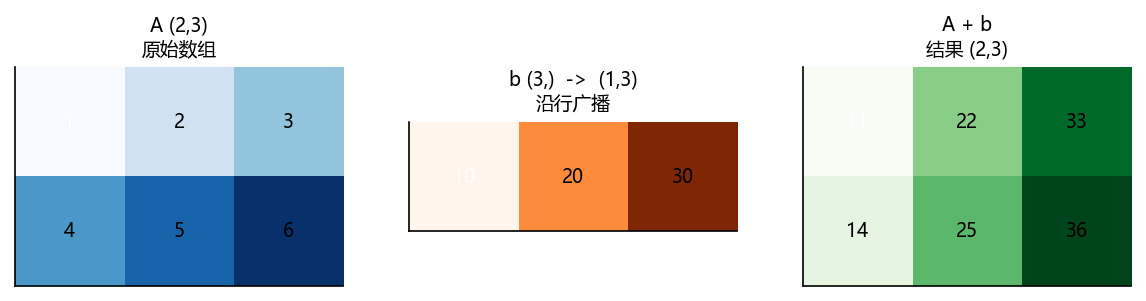
\includegraphics[keepaspectratio,alt={广播示意图}]{figures/01-numpy/broadcast.png}}
\caption{广播示意图}
\end{figure}

\begin{itemize}
\tightlist
\item
  \texttt{(2,3)\ +\ (3,)} √，结果为 \texttt{(2,3)}；
\item
  \texttt{(3,)\ +\ (4,)} ×（末尾不等且无 1）；
\item
  \texttt{(4,1)\ +\ (1,3)} √，结果 \texttt{(4,3)}；
\item
  \texttt{(4,1,6)\ +\ (3,6)} √，结果 \texttt{(4,3,6)}（把 \texttt{(3,6)}
  补成 \texttt{(1,3,6)}）。
\end{itemize}

\textbf{调试技巧}：报错时打印两个数组的 \texttt{shape}，用
\texttt{np.newaxis}（即 \texttt{None}）手动补维。

\begin{center}\rule{0.5\linewidth}{0.5pt}\end{center}

\subsection{1.7
随机数生成与抽样}\label{ux968fux673aux6570ux751fux6210ux4e0eux62bdux6837}

\subsubsection{1.7.1
新版推荐：Generator}\label{ux65b0ux7248ux63a8ux8350generator}

\begin{Shaded}
\begin{Highlighting}[]
\NormalTok{rng }\OperatorTok{=}\NormalTok{ np.random.default\_rng(}\DecValTok{42}\NormalTok{)      }\CommentTok{\# 固定种子，结果可复现}
\NormalTok{rng.random((}\DecValTok{2}\NormalTok{, }\DecValTok{3}\NormalTok{))                   }\CommentTok{\# [0,1) 均匀}
\NormalTok{rng.integers(}\DecValTok{1}\NormalTok{, }\DecValTok{10}\NormalTok{, size}\OperatorTok{=}\DecValTok{5}\NormalTok{)          }\CommentTok{\# 整数 [1,10)}
\NormalTok{rng.uniform(}\OperatorTok{{-}}\DecValTok{1}\NormalTok{, }\DecValTok{1}\NormalTok{, size}\OperatorTok{=}\DecValTok{4}\NormalTok{)           }\CommentTok{\# 均匀分布}
\NormalTok{rng.normal(}\DecValTok{2}\NormalTok{, }\FloatTok{0.5}\NormalTok{, size}\OperatorTok{=}\DecValTok{6}\NormalTok{)           }\CommentTok{\# 正态 N(2, 0.5\^{}2)}
\end{Highlighting}
\end{Shaded}

\subsubsection{1.7.2
旧接口（仍可用，但不建议用于新代码）}\label{ux65e7ux63a5ux53e3ux4ecdux53efux7528ux4f46ux4e0dux5efaux8baeux7528ux4e8eux65b0ux4ee3ux7801}

\begin{Shaded}
\begin{Highlighting}[]
\NormalTok{np.random.seed(}\DecValTok{42}\NormalTok{)}
\NormalTok{np.random.rand(}\DecValTok{2}\NormalTok{, }\DecValTok{3}\NormalTok{)     }\CommentTok{\# [0,1)}
\NormalTok{np.random.randint(}\DecValTok{1}\NormalTok{, }\DecValTok{10}\NormalTok{) }\CommentTok{\# 整数}
\NormalTok{np.random.randn(}\DecValTok{5}\NormalTok{)       }\CommentTok{\# 标准正态}
\NormalTok{np.random.normal(}\DecValTok{2}\NormalTok{, }\FloatTok{0.5}\NormalTok{, }\DecValTok{5}\NormalTok{)}
\end{Highlighting}
\end{Shaded}

\textbf{选型}：新代码优先
\texttt{default\_rng}（更快、线程安全、接口清晰）。

\begin{center}\rule{0.5\linewidth}{0.5pt}\end{center}

\subsection{常见误区}\label{ux5e38ux89c1ux8befux533a}

\begin{enumerate}
\def\labelenumi{\arabic{enumi}.}
\tightlist
\item
  \textbf{\texttt{*} 不等于矩阵乘法}：\texttt{A\ *\ B}
  是逐元素乘法；矩阵乘法用 \texttt{A\ @\ B} 或 \texttt{np.matmul}。
\item
  \textbf{忘记 \texttt{zeros/ones/full}
  要传元组}：\texttt{np.zeros(2,\ 3)} 会报错，应为
  \texttt{np.zeros((2,\ 3))}。
\item
  \textbf{以为 \texttt{reshape}
  一定返回拷贝}：连续内存下是视图；改视图会影响原数组。
\item
  \textbf{误用
  \texttt{len(a)}}：一维数组返回长度，二维返回行数；看形状用
  \texttt{a.shape}。
\item
  \textbf{广播不通用}：\texttt{(3,)\ +\ (4,)} 不会自动``截断对齐''。
\item
  \textbf{随机数不设种子}：不设种子结果每次不同，课堂演示/作业请用
  \texttt{default\_rng(seed)}。
\end{enumerate}

\subsection{思考题}\label{ux601dux8003ux9898}

\begin{enumerate}
\def\labelenumi{\arabic{enumi}.}
\tightlist
\item
  \texttt{np.arange(10){[}::2{]}} 与
  \texttt{np.arange(10).reshape(5,2){[}:,0{]}} 是否共享内存？用
  `\texttt{.base} 验证。
\item
  解释 \texttt{np.ix\_} 与同时传入两个顺序索引的区别。
\item
  举一个形状满足广播规则却``符合直觉但结果错误''的例子（提示：\texttt{(3,1)}
  与 \texttt{(3,)}）。
\end{enumerate}

\subsection{动手练习（详见
lab）}\label{ux52a8ux624bux7ec3ux4e60ux8be6ux89c1-lab}

\begin{itemize}
\tightlist
\item
  创建 3×4 矩阵，用布尔掩码把负数置 0；
\item
  用 \texttt{np.arange} 生成 0--100 的偶数，转成 10×5 矩阵；
\item
  复现``对每列做不同缩放''的广播例子；
\item
  用 \texttt{default\_rng(0)} 生成 100 个标准正态数并统计均值/方差。
\end{itemize}

\subsection{延伸阅读}\label{ux5ef6ux4f38ux9605ux8bfb}

\begin{itemize}
\tightlist
\item
  NumPy
  官方绝对入门：https://numpy.org/doc/stable/user/absolute\_beginners.html
\item
  NumPy
  官方广播机制：https://numpy.org/doc/stable/user/basics.broadcasting.html
\item
  SciPy Lecture Notes --
  NumPy：https://scipy-lectures.org/intro/numpy/index.html
\end{itemize}

\section{02
数组运算：向量、矩阵、逻辑筛选与统计}\label{ux6570ux7ec4ux8fd0ux7b97ux5411ux91cfux77e9ux9635ux903bux8f91ux7b5bux9009ux4e0eux7edfux8ba1}

\begin{quote}
本节对应原版 1.2 的内容，并增补学习目标、常见误区、思考题与延伸阅读。
配套图：\texttt{figures/01-numpy/vector\_ops.png}。
\end{quote}

\subsection{本节目标}\label{ux672cux8282ux76eeux6807-1}

\begin{itemize}
\tightlist
\item
  区分\textbf{逐元素运算}与\textbf{线性代数运算}（\texttt{*} vs
  \texttt{@} / \texttt{dot}）；
\item
  会用布尔掩码与 \texttt{np.where} 做筛选与替换；
\item
  掌握 \texttt{sum/mean/std/min/max} 沿 \texttt{axis} 方向统计；
\item
  会用 \texttt{sort/argsort} 排序与排名；
\item
  会用
  \texttt{savetxt/loadtxt}、\texttt{save/load}、\texttt{savez\_compressed}
  保存与读取数组。
\end{itemize}

\subsection{先修}\label{ux5148ux4fee-1}

\begin{itemize}
\tightlist
\item
  01 数组基础（创建、索引、广播）。
\end{itemize}

\begin{center}\rule{0.5\linewidth}{0.5pt}\end{center}

\subsection{2.1 向量的运算}\label{ux5411ux91cfux7684ux8fd0ux7b97}

\subsubsection{2.1.1 逐元素操作}\label{ux9010ux5143ux7d20ux64cdux4f5c}

\begin{Shaded}
\begin{Highlighting}[]
\ImportTok{import}\NormalTok{ numpy }\ImportTok{as}\NormalTok{ np}

\NormalTok{v }\OperatorTok{=}\NormalTok{ np.array([}\DecValTok{2}\NormalTok{, }\DecValTok{3}\NormalTok{])}
\NormalTok{w }\OperatorTok{=}\NormalTok{ np.array([}\DecValTok{3}\NormalTok{, }\DecValTok{1}\NormalTok{])}
\BuiltInTok{print}\NormalTok{(v }\OperatorTok{+}\NormalTok{ w)     }\CommentTok{\# [5 4]}
\BuiltInTok{print}\NormalTok{(v }\OperatorTok{{-}}\NormalTok{ w)     }\CommentTok{\# [{-}1  2]}
\BuiltInTok{print}\NormalTok{(}\DecValTok{2} \OperatorTok{*}\NormalTok{ v)     }\CommentTok{\# [4 6]}
\BuiltInTok{print}\NormalTok{(v }\OperatorTok{*}\NormalTok{ w)     }\CommentTok{\# 逐元素乘 [6 3]}
\BuiltInTok{print}\NormalTok{(v }\OperatorTok{/}\NormalTok{ w)     }\CommentTok{\# 逐元素除 [0.66666667 3.        ]}
\BuiltInTok{print}\NormalTok{(v }\OperatorTok{**} \DecValTok{2}\NormalTok{)    }\CommentTok{\# 逐元素平方 [4 9]}
\end{Highlighting}
\end{Shaded}

\begin{figure}
\centering
\pandocbounded{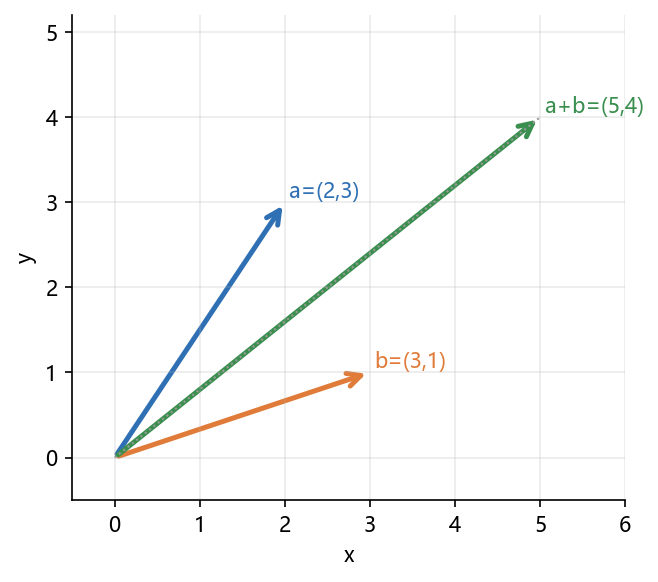
\includegraphics[keepaspectratio,alt={向量运算示意}]{figures/01-numpy/vector_ops.png}}
\caption{向量运算示意}
\end{figure}

\subsubsection{2.1.2
数量积（点积）与叉积}\label{ux6570ux91cfux79efux70b9ux79efux4e0eux53c9ux79ef}

\begin{Shaded}
\begin{Highlighting}[]
\NormalTok{a }\OperatorTok{=}\NormalTok{ np.array([}\DecValTok{1}\NormalTok{, }\DecValTok{2}\NormalTok{])}
\NormalTok{b }\OperatorTok{=}\NormalTok{ np.array([}\DecValTok{3}\NormalTok{, }\DecValTok{4}\NormalTok{])}
\BuiltInTok{print}\NormalTok{(np.dot(a, b))      }\CommentTok{\# 1*3 + 2*4 = 11}
\BuiltInTok{print}\NormalTok{(a }\OperatorTok{@}\NormalTok{ b)             }\CommentTok{\# 向量点积同样可用 @}

\NormalTok{c }\OperatorTok{=}\NormalTok{ np.array([}\DecValTok{1}\NormalTok{, }\DecValTok{2}\NormalTok{, }\DecValTok{3}\NormalTok{])}
\NormalTok{d }\OperatorTok{=}\NormalTok{ np.array([}\DecValTok{4}\NormalTok{, }\DecValTok{5}\NormalTok{, }\DecValTok{6}\NormalTok{])}
\BuiltInTok{print}\NormalTok{(np.cross(c, d))    }\CommentTok{\# [{-}3  6 {-}3]}
\end{Highlighting}
\end{Shaded}

\subsubsection{2.1.3 向量的范数}\label{ux5411ux91cfux7684ux8303ux6570}

\begin{Shaded}
\begin{Highlighting}[]
\NormalTok{x }\OperatorTok{=}\NormalTok{ np.array([}\DecValTok{3}\NormalTok{, }\DecValTok{4}\NormalTok{])}
\NormalTok{np.linalg.norm(x)        }\CommentTok{\# 5.0（默认 2{-}范数）}
\NormalTok{np.linalg.norm(x, }\BuiltInTok{ord}\OperatorTok{=}\DecValTok{1}\NormalTok{) }\CommentTok{\# 7.0（1{-}范数）}
\end{Highlighting}
\end{Shaded}

\subsubsection{2.1.4 排序}\label{ux6392ux5e8f}

\begin{Shaded}
\begin{Highlighting}[]
\NormalTok{a }\OperatorTok{=}\NormalTok{ np.array([}\DecValTok{3}\NormalTok{, }\DecValTok{1}\NormalTok{, }\DecValTok{2}\NormalTok{])}
\NormalTok{np.sort(a)          }\CommentTok{\# 返回新数组 [1 2 3]}
\NormalTok{a.sort()            }\CommentTok{\# 原地排序}
\NormalTok{np.argsort(a)       }\CommentTok{\# 排序后原索引}
\end{Highlighting}
\end{Shaded}

\begin{center}\rule{0.5\linewidth}{0.5pt}\end{center}

\subsection{2.2
向量/矩阵的逻辑运算------筛选}\label{ux5411ux91cfux77e9ux9635ux7684ux903bux8f91ux8fd0ux7b97ux7b5bux9009}

\begin{Shaded}
\begin{Highlighting}[]
\NormalTok{x }\OperatorTok{=}\NormalTok{ np.array([}\DecValTok{1}\NormalTok{, }\OperatorTok{{-}}\DecValTok{2}\NormalTok{, }\DecValTok{3}\NormalTok{, }\OperatorTok{{-}}\DecValTok{4}\NormalTok{, }\DecValTok{5}\NormalTok{])}

\CommentTok{\#\# 布尔掩码}
\BuiltInTok{print}\NormalTok{(x[x }\OperatorTok{\textgreater{}} \DecValTok{0}\NormalTok{])          }\CommentTok{\# [1 3 5]}
\BuiltInTok{print}\NormalTok{(x[(x }\OperatorTok{\textgreater{}} \DecValTok{1}\NormalTok{) }\OperatorTok{\&}\NormalTok{ (x }\OperatorTok{\textless{}} \DecValTok{5}\NormalTok{)])  }\CommentTok{\# [3]}

\CommentTok{\#\# np.where：条件成立取第一项，否则取第二项}
\BuiltInTok{print}\NormalTok{(np.where(x }\OperatorTok{\textgreater{}} \DecValTok{0}\NormalTok{, x, }\DecValTok{0}\NormalTok{))   }\CommentTok{\# [1 0 3 0 5]}
\end{Highlighting}
\end{Shaded}

二维按行筛选：

\begin{Shaded}
\begin{Highlighting}[]
\NormalTok{m }\OperatorTok{=}\NormalTok{ np.array([[}\DecValTok{1}\NormalTok{, }\DecValTok{9}\NormalTok{], [}\DecValTok{6}\NormalTok{, }\DecValTok{2}\NormalTok{], [}\DecValTok{7}\NormalTok{, }\DecValTok{8}\NormalTok{]])}
\BuiltInTok{print}\NormalTok{(m[(m[:, }\DecValTok{0}\NormalTok{] }\OperatorTok{\textgreater{}} \DecValTok{3}\NormalTok{) }\OperatorTok{\&}\NormalTok{ (m[:, }\DecValTok{1}\NormalTok{] }\OperatorTok{\textless{}} \DecValTok{9}\NormalTok{)])   }\CommentTok{\# [[6 2] [7 8]]}
\end{Highlighting}
\end{Shaded}

\begin{quote}
组合条件必须加括号，且不能用 \texttt{and} / \texttt{or}，要用
\texttt{\&} / \texttt{\textbar{}} / \texttt{\textasciitilde{}}。
\end{quote}

\begin{center}\rule{0.5\linewidth}{0.5pt}\end{center}

\subsection{2.3 矩阵的运算}\label{ux77e9ux9635ux7684ux8fd0ux7b97}

\subsubsection{2.3.1 算术运算}\label{ux7b97ux672fux8fd0ux7b97}

\begin{Shaded}
\begin{Highlighting}[]
\NormalTok{A }\OperatorTok{=}\NormalTok{ np.array([[}\DecValTok{1}\NormalTok{, }\DecValTok{2}\NormalTok{], [}\DecValTok{3}\NormalTok{, }\DecValTok{4}\NormalTok{]])}
\NormalTok{B }\OperatorTok{=}\NormalTok{ np.array([[}\DecValTok{5}\NormalTok{, }\DecValTok{6}\NormalTok{], [}\DecValTok{7}\NormalTok{, }\DecValTok{8}\NormalTok{]])}

\BuiltInTok{print}\NormalTok{(A }\OperatorTok{+}\NormalTok{ B)      }\CommentTok{\# 矩阵加法 [[ 6  8][10 12]]}
\BuiltInTok{print}\NormalTok{(A }\OperatorTok{{-}}\NormalTok{ B)      }\CommentTok{\# 矩阵减法}
\BuiltInTok{print}\NormalTok{(A }\OperatorTok{*}\NormalTok{ B)      }\CommentTok{\# 注意：逐元素乘 [[ 5 12][21 32]]}
\BuiltInTok{print}\NormalTok{(A }\OperatorTok{@}\NormalTok{ B)      }\CommentTok{\# √ 矩阵乘 [[19 22][43 50]]}
\BuiltInTok{print}\NormalTok{(np.matmul(A, B))   }\CommentTok{\# 同 @}
\end{Highlighting}
\end{Shaded}

\textbf{为什么 \texttt{*} 不是矩阵乘}：NumPy 中 \texttt{*} 是
\texttt{ufunc} 的逐元素运算；要数学上的矩阵乘法，用 \texttt{@}（或
\texttt{np.dot} / \texttt{np.matmul}，二者在 2D 下等价，但 \texttt{@}
语义更明确）。

\subsubsection{2.3.2
矩阵上的统计}\label{ux77e9ux9635ux4e0aux7684ux7edfux8ba1}

\begin{Shaded}
\begin{Highlighting}[]
\NormalTok{S }\OperatorTok{=}\NormalTok{ np.array([[}\DecValTok{85}\NormalTok{, }\DecValTok{90}\NormalTok{, }\DecValTok{80}\NormalTok{],}
\NormalTok{              [}\DecValTok{78}\NormalTok{, }\DecValTok{85}\NormalTok{, }\DecValTok{90}\NormalTok{],}
\NormalTok{              [}\DecValTok{90}\NormalTok{, }\DecValTok{95}\NormalTok{, }\DecValTok{85}\NormalTok{]])}

\NormalTok{S.}\BuiltInTok{sum}\NormalTok{(axis}\OperatorTok{=}\DecValTok{0}\NormalTok{)      }\CommentTok{\# 每列和 [253 270 255]（三门课总分）}
\NormalTok{S.}\BuiltInTok{sum}\NormalTok{(axis}\OperatorTok{=}\DecValTok{1}\NormalTok{)      }\CommentTok{\# 每行和 [255 253 270]（每个学生总分）}
\NormalTok{S.mean(axis}\OperatorTok{=}\DecValTok{0}\NormalTok{)     }\CommentTok{\# 每列均值 [84.33 90. 85. ]}
\NormalTok{S.}\BuiltInTok{max}\NormalTok{(axis}\OperatorTok{=}\DecValTok{1}\NormalTok{)      }\CommentTok{\# 每行最大值}
\NormalTok{S.std()            }\CommentTok{\# 全体标准差}
\end{Highlighting}
\end{Shaded}

记忆：\texttt{axis=0} 表示``沿第 0
轴（行方向）折叠''，即求\textbf{每列}的统计量；\texttt{axis=1}
求\textbf{每行}。

\subsubsection{2.3.3 查找（where /
argmax）}\label{ux67e5ux627ewhere-argmax}

\begin{Shaded}
\begin{Highlighting}[]
\NormalTok{m }\OperatorTok{=}\NormalTok{ np.array([[}\DecValTok{3}\NormalTok{, }\DecValTok{7}\NormalTok{], [}\DecValTok{9}\NormalTok{, }\DecValTok{2}\NormalTok{]])}
\NormalTok{np.where(m }\OperatorTok{\textgreater{}} \DecValTok{5}\NormalTok{)          }\CommentTok{\# (array([0,1]), array([1,0])) 坐标}
\NormalTok{np.argmax(m)             }\CommentTok{\# 展平后的最大索引 2 → (1,0)}
\NormalTok{np.argmax(m, axis}\OperatorTok{=}\DecValTok{1}\NormalTok{)     }\CommentTok{\# 每行最大索引 [1 0]}
\end{Highlighting}
\end{Shaded}

\begin{center}\rule{0.5\linewidth}{0.5pt}\end{center}

\subsection{2.4
结果的保存与读取}\label{ux7ed3ux679cux7684ux4fddux5b58ux4e0eux8bfbux53d6}

\begin{Shaded}
\begin{Highlighting}[]
\NormalTok{a }\OperatorTok{=}\NormalTok{ np.array([[}\DecValTok{1}\NormalTok{, }\DecValTok{2}\NormalTok{], [}\DecValTok{3}\NormalTok{, }\DecValTok{4}\NormalTok{]])}

\CommentTok{\#\# 文本}
\NormalTok{np.savetxt(}\StringTok{"result.txt"}\NormalTok{, a, fmt}\OperatorTok{=}\StringTok{"}\SpecialCharTok{\%.2f}\StringTok{"}\NormalTok{, delimiter}\OperatorTok{=}\StringTok{","}\NormalTok{)}
\NormalTok{b }\OperatorTok{=}\NormalTok{ np.loadtxt(}\StringTok{"result.txt"}\NormalTok{, delimiter}\OperatorTok{=}\StringTok{","}\NormalTok{)}

\CommentTok{\#\# 二进制（推荐：更快、保留 dtype）}
\NormalTok{np.save(}\StringTok{"a.npy"}\NormalTok{, a)}
\NormalTok{c }\OperatorTok{=}\NormalTok{ np.load(}\StringTok{"a.npy"}\NormalTok{)}

\CommentTok{\#\# 多数组压缩保存}
\NormalTok{np.savez\_compressed(}\StringTok{"data.npz"}\NormalTok{, x}\OperatorTok{=}\NormalTok{a, y}\OperatorTok{=}\NormalTok{b)}
\NormalTok{d }\OperatorTok{=}\NormalTok{ np.load(}\StringTok{"data.npz"}\NormalTok{)}
\NormalTok{d[}\StringTok{"x"}\NormalTok{], d[}\StringTok{"y"}\NormalTok{]}
\end{Highlighting}
\end{Shaded}

\begin{center}\rule{0.5\linewidth}{0.5pt}\end{center}

\subsection{常见误区}\label{ux5e38ux89c1ux8befux533a-1}

\begin{enumerate}
\def\labelenumi{\arabic{enumi}.}
\tightlist
\item
  \textbf{\texttt{*} 与 \texttt{@} 混用}：\texttt{A\ *\ B}
  是逐元素乘；数学矩阵乘必须 \texttt{@}。
\item
  \textbf{axis 方向记反}：\texttt{sum(axis=0)} 是``消除第 0
  维''，得到每列结果。
\item
  \textbf{条件用 \texttt{and}/\texttt{or}}：数组布尔运算必须
  \texttt{\&}/\texttt{\textbar{}}，且每个条件加括号。
\item
  \textbf{反复
  \texttt{np.append}}：每次产生新数组，大数组循环中极慢；先估算容量或用列表。
\item
  \textbf{\texttt{np.dot} 语义在多维下容易混淆}：明确用 \texttt{@}
  更直观。
\end{enumerate}

\subsection{思考题}\label{ux601dux8003ux9898-1}

\begin{enumerate}
\def\labelenumi{\arabic{enumi}.}
\tightlist
\item
  \texttt{np.dot}、\texttt{np.matmul}、\texttt{@}
  在三维数组上行为是否一致？查文档说明。
\item
  为什么 \texttt{np.where(cond,\ x,\ y)} 要求 \texttt{x}、\texttt{y}
  可广播到 \texttt{cond} 的形状？
\item
  用 \texttt{argsort} 给三位学生按总分排名。
\end{enumerate}

\subsection{动手练习（详见
lab）}\label{ux52a8ux624bux7ec3ux4e60ux8be6ux89c1-lab-1}

\begin{itemize}
\tightlist
\item
  生成 5×5 随机矩阵，把主对角线元素置 0；
\item
  对每列做 z-score 标准化（\texttt{(x\ -\ mean)\ /\ std}），并比较
  \texttt{axis} 的选择；
\item
  用 \texttt{savetxt}/\texttt{loadtxt} 存取一份成绩表并检查数值一致。
\end{itemize}

\subsection{延伸阅读}\label{ux5ef6ux4f38ux9605ux8bfb-1}

\begin{itemize}
\tightlist
\item
  NumPy 官方 ndarray
  基础：https://numpy.org/doc/stable/user/quickstart.html
\item
  NumPy 官方 I/O
  说明：https://numpy.org/doc/stable/reference/routines.io.html
\item
  SciPy Lecture Notes --
  数组操作：https://scipy-lectures.org/intro/numpy/operations.html
\end{itemize}

\section{03 线性代数：逆、方程组、分解与
SVD}\label{ux7ebfux6027ux4ee3ux6570ux9006ux65b9ux7a0bux7ec4ux5206ux89e3ux4e0e-svd}

\begin{quote}
本节对应原版 1.3 的内容，并增补学习目标、常见误区、思考题与延伸阅读。
配套图：\texttt{figures/01-numpy/cond\_sensitivity.png}、\texttt{figures/01-numpy/svd\_compression.png}。
\end{quote}

\subsection{本节目标}\label{ux672cux8282ux76eeux6807-2}

\begin{itemize}
\tightlist
\item
  会求逆矩阵、伪逆、秩、行列式、范数；
\item
  会用 \texttt{np.linalg.solve} 解线性方程组，理解条件数（condition
  number）对数值稳定的影响；
\item
  会用 \texttt{np.linalg.lstsq} 做最小二乘；
\item
  掌握特征值分解、SVD、Cholesky、QR 分解的基本用法与适用场景；
\item
  能说出 SVD 的``压缩/降维''思想（见 05 综合案例）。
\end{itemize}

\subsection{先修}\label{ux5148ux4fee-2}

\begin{itemize}
\tightlist
\item
  01 数组基础、02 数组运算；线性代数的基本概念（矩阵、行列式、特征值）。
\end{itemize}

\begin{center}\rule{0.5\linewidth}{0.5pt}\end{center}

\subsection{3.1
基本线性代数运算}\label{ux57faux672cux7ebfux6027ux4ee3ux6570ux8fd0ux7b97}

\subsubsection{3.1.1
逆矩阵与伪逆}\label{ux9006ux77e9ux9635ux4e0eux4f2aux9006}

\begin{Shaded}
\begin{Highlighting}[]
\ImportTok{import}\NormalTok{ numpy }\ImportTok{as}\NormalTok{ np}

\NormalTok{A }\OperatorTok{=}\NormalTok{ np.array([[}\DecValTok{3}\NormalTok{, }\DecValTok{1}\NormalTok{], [}\DecValTok{1}\NormalTok{, }\DecValTok{2}\NormalTok{]])}
\NormalTok{A\_inv }\OperatorTok{=}\NormalTok{ np.linalg.inv(A)}
\BuiltInTok{print}\NormalTok{(A\_inv)}
\CommentTok{\#\# [[ 0.4 {-}0.2]}
\CommentTok{\#\#  [{-}0.2  0.6]]}
\BuiltInTok{print}\NormalTok{(A }\OperatorTok{@}\NormalTok{ A\_inv)      }\CommentTok{\# ≈ 单位矩阵}
\end{Highlighting}
\end{Shaded}

非方阵或奇异矩阵用 \texttt{pinv}（伪逆），常用于最小二乘与超定方程组：

\begin{Shaded}
\begin{Highlighting}[]
\NormalTok{B }\OperatorTok{=}\NormalTok{ np.array([[}\DecValTok{1}\NormalTok{, }\DecValTok{2}\NormalTok{], [}\DecValTok{2}\NormalTok{, }\DecValTok{4}\NormalTok{], [}\DecValTok{3}\NormalTok{, }\DecValTok{6}\NormalTok{]])   }\CommentTok{\# 秩亏}
\BuiltInTok{print}\NormalTok{(np.linalg.pinv(B).shape)           }\CommentTok{\# (2,3)}
\end{Highlighting}
\end{Shaded}

\subsubsection{3.1.2 秩}\label{ux79e9}

\begin{Shaded}
\begin{Highlighting}[]
\NormalTok{np.linalg.matrix\_rank(np.array([[}\DecValTok{1}\NormalTok{, }\DecValTok{2}\NormalTok{], [}\DecValTok{2}\NormalTok{, }\DecValTok{4}\NormalTok{]]))   }\CommentTok{\# 1（第二行是第一行的 2 倍）}
\NormalTok{np.linalg.matrix\_rank(np.array([[}\DecValTok{1}\NormalTok{, }\DecValTok{2}\NormalTok{], [}\DecValTok{3}\NormalTok{, }\DecValTok{4}\NormalTok{]]))   }\CommentTok{\# 2}
\end{Highlighting}
\end{Shaded}

\subsubsection{3.1.3 行列式}\label{ux884cux5217ux5f0f}

\begin{Shaded}
\begin{Highlighting}[]
\NormalTok{A }\OperatorTok{=}\NormalTok{ np.array([[}\DecValTok{3}\NormalTok{, }\DecValTok{1}\NormalTok{], [}\DecValTok{1}\NormalTok{, }\DecValTok{2}\NormalTok{]])}
\BuiltInTok{print}\NormalTok{(np.linalg.det(A))    }\CommentTok{\# 5.0（近似）}
\end{Highlighting}
\end{Shaded}

行列式为 0 等价于矩阵奇异，此时方程组没有唯一解。

\subsubsection{3.1.4 范数}\label{ux8303ux6570}

\begin{Shaded}
\begin{Highlighting}[]
\NormalTok{v }\OperatorTok{=}\NormalTok{ np.array([}\DecValTok{3}\NormalTok{, }\DecValTok{4}\NormalTok{])}
\NormalTok{np.linalg.norm(v)              }\CommentTok{\# 5.0，2{-}范数}
\NormalTok{np.linalg.norm(v, }\BuiltInTok{ord}\OperatorTok{=}\DecValTok{1}\NormalTok{)       }\CommentTok{\# 7.0}

\NormalTok{M }\OperatorTok{=}\NormalTok{ np.array([[}\DecValTok{3}\NormalTok{, }\DecValTok{4}\NormalTok{], [}\DecValTok{0}\NormalTok{, }\DecValTok{5}\NormalTok{]])}
\NormalTok{np.linalg.norm(M)              }\CommentTok{\# Frobenius 范数 ≈ 7.0711}
\NormalTok{np.linalg.norm(M, }\BuiltInTok{ord}\OperatorTok{=}\DecValTok{2}\NormalTok{)       }\CommentTok{\# 谱范数（最大奇异值）}
\NormalTok{np.linalg.norm(M, }\BuiltInTok{ord}\OperatorTok{=}\NormalTok{np.inf)  }\CommentTok{\# 无穷范数（行和最大值）}
\end{Highlighting}
\end{Shaded}

\begin{center}\rule{0.5\linewidth}{0.5pt}\end{center}

\subsection{3.2
线性方程组的求解}\label{ux7ebfux6027ux65b9ux7a0bux7ec4ux7684ux6c42ux89e3}

\subsubsection{\texorpdfstring{3.2.1
直接求解：\texttt{np.linalg.solve}}{3.2.1 直接求解：np.linalg.solve}}\label{ux76f4ux63a5ux6c42ux89e3np.linalg.solve}

\begin{Shaded}
\begin{Highlighting}[]
\NormalTok{A }\OperatorTok{=}\NormalTok{ np.array([[}\DecValTok{3}\NormalTok{, }\DecValTok{1}\NormalTok{], [}\DecValTok{1}\NormalTok{, }\DecValTok{2}\NormalTok{]])   }\CommentTok{\# 系数矩阵}
\NormalTok{b }\OperatorTok{=}\NormalTok{ np.array([}\DecValTok{9}\NormalTok{, }\DecValTok{8}\NormalTok{])             }\CommentTok{\# 常数向量}
\NormalTok{x }\OperatorTok{=}\NormalTok{ np.linalg.solve(A, b)}
\BuiltInTok{print}\NormalTok{(x)          }\CommentTok{\# [2. 3.]，即 x=2, y=3}
\BuiltInTok{print}\NormalTok{(A }\OperatorTok{@}\NormalTok{ x)      }\CommentTok{\# ≈ [9. 8.]}
\end{Highlighting}
\end{Shaded}

\textbf{适用条件}：\texttt{A}
是方阵且非奇异（存在唯一解）。结构更一般的线性方程组用 \texttt{lstsq}。

\subsubsection{\texorpdfstring{3.2.2
最小二乘：\texttt{np.linalg.lstsq}}{3.2.2 最小二乘：np.linalg.lstsq}}\label{ux6700ux5c0fux4e8cux4e58np.linalg.lstsq}

超定（方程多于未知数）或欠定（方程少于未知数）时，求``误差平方和最小''的解：

\begin{Shaded}
\begin{Highlighting}[]
\NormalTok{X }\OperatorTok{=}\NormalTok{ np.array([[}\DecValTok{1}\NormalTok{, }\DecValTok{1}\NormalTok{], [}\DecValTok{1}\NormalTok{, }\DecValTok{2}\NormalTok{], [}\DecValTok{1}\NormalTok{, }\DecValTok{3}\NormalTok{], [}\DecValTok{1}\NormalTok{, }\DecValTok{4}\NormalTok{]])}
\NormalTok{y }\OperatorTok{=}\NormalTok{ np.array([}\DecValTok{6}\NormalTok{, }\DecValTok{5}\NormalTok{, }\DecValTok{7}\NormalTok{, }\DecValTok{10}\NormalTok{])}
\NormalTok{coef, residuals, rank, sv }\OperatorTok{=}\NormalTok{ np.linalg.lstsq(X, y, rcond}\OperatorTok{=}\VariableTok{None}\NormalTok{)}
\BuiltInTok{print}\NormalTok{(coef)      }\CommentTok{\# [3.5 1.4] → y ≈ 3.5 + 1.4 x}
\end{Highlighting}
\end{Shaded}

\subsubsection{3.2.3
条件数与数值稳定性}\label{ux6761ux4ef6ux6570ux4e0eux6570ux503cux7a33ux5b9aux6027}

条件数 \texttt{cond(A)}
刻画方程组对扰动的敏感程度：条件数越大，解越``脆弱''。

\begin{Shaded}
\begin{Highlighting}[]
\NormalTok{A }\OperatorTok{=}\NormalTok{ np.array([[}\DecValTok{1}\NormalTok{, }\DecValTok{2}\NormalTok{, }\DecValTok{3}\NormalTok{],}
\NormalTok{              [}\DecValTok{2}\NormalTok{, }\FloatTok{4.0001}\NormalTok{, }\DecValTok{6}\NormalTok{],}
\NormalTok{              [}\DecValTok{1}\NormalTok{, }\FloatTok{0.9999}\NormalTok{, }\DecValTok{2}\NormalTok{]])}
\NormalTok{b }\OperatorTok{=}\NormalTok{ np.array([}\DecValTok{1}\NormalTok{, }\DecValTok{2}\NormalTok{, }\DecValTok{3}\NormalTok{])}
\BuiltInTok{print}\NormalTok{(np.linalg.cond(A))   }\CommentTok{\# 这个矩阵近似奇异，cond 很大}
\NormalTok{x0 }\OperatorTok{=}\NormalTok{ np.linalg.solve(A, b)}
\end{Highlighting}
\end{Shaded}

\begin{figure}
\centering
\pandocbounded{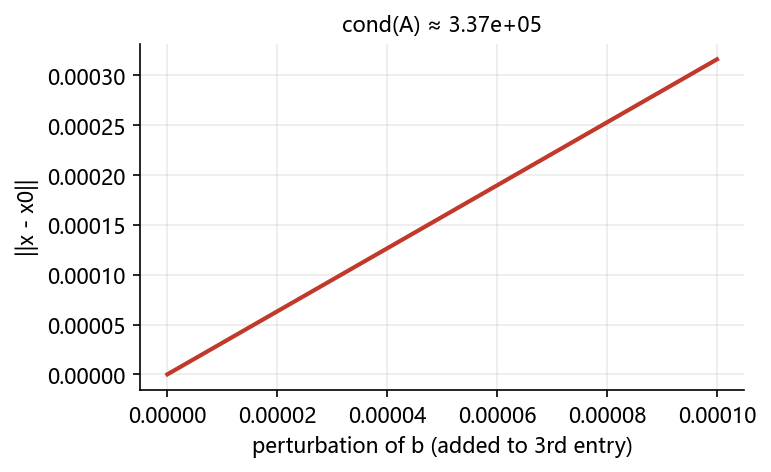
\includegraphics[keepaspectratio,alt={条件数敏感性}]{figures/01-numpy/cond_sensitivity.png}}
\caption{条件数敏感性}
\end{figure}

\textbf{结论}：即使 \texttt{b} 的扰动非常小（\texttt{1e-4}
量级），解的变化也可能很大；工程中应尽量避免病态方程组，或换用更稳定的分解方法。

\begin{center}\rule{0.5\linewidth}{0.5pt}\end{center}

\subsection{3.3 矩阵分解}\label{ux77e9ux9635ux5206ux89e3}

\subsubsection{\texorpdfstring{3.3.1
特征值分解（\texttt{eig}）}{3.3.1 特征值分解（eig）}}\label{ux7279ux5f81ux503cux5206ux89e3eig}

只适用于\textbf{方阵}（且通常要求可对角化）：

\begin{Shaded}
\begin{Highlighting}[]
\NormalTok{A }\OperatorTok{=}\NormalTok{ np.array([[}\DecValTok{2}\NormalTok{, }\DecValTok{1}\NormalTok{], [}\DecValTok{1}\NormalTok{, }\DecValTok{2}\NormalTok{]])}
\NormalTok{w, v }\OperatorTok{=}\NormalTok{ np.linalg.eig(A)}
\BuiltInTok{print}\NormalTok{(w)          }\CommentTok{\# [3. 1.] 特征值}
\BuiltInTok{print}\NormalTok{(v)          }\CommentTok{\# 列向量为对应特征向量}
\BuiltInTok{print}\NormalTok{(A }\OperatorTok{@}\NormalTok{ v[:, }\DecValTok{0}\NormalTok{] }\OperatorTok{==}\NormalTok{ w[}\DecValTok{0}\NormalTok{] }\OperatorTok{*}\NormalTok{ v[:, }\DecValTok{0}\NormalTok{])   }\CommentTok{\# 验证 Av = λv}
\end{Highlighting}
\end{Shaded}

\subsubsection{3.3.2
奇异值分解（SVD）}\label{ux5947ux5f02ux503cux5206ux89e3svd}

对\textbf{任意矩阵}（包括非方阵）适用：

\begin{Shaded}
\begin{Highlighting}[]
\NormalTok{M }\OperatorTok{=}\NormalTok{ np.array([[}\DecValTok{1}\NormalTok{, }\DecValTok{2}\NormalTok{], [}\DecValTok{3}\NormalTok{, }\DecValTok{4}\NormalTok{], [}\DecValTok{5}\NormalTok{, }\DecValTok{6}\NormalTok{]], dtype}\OperatorTok{=}\BuiltInTok{float}\NormalTok{)}
\NormalTok{U, S, Vt }\OperatorTok{=}\NormalTok{ np.linalg.svd(M, full\_matrices}\OperatorTok{=}\VariableTok{False}\NormalTok{)}
\BuiltInTok{print}\NormalTok{(U.shape, S.shape, Vt.shape)   }\CommentTok{\# (3,2) (2,) (2,2)}
\BuiltInTok{print}\NormalTok{(S)                            }\CommentTok{\# 奇异值（降序）}
\BuiltInTok{print}\NormalTok{(U }\OperatorTok{@}\NormalTok{ np.diag(S) }\OperatorTok{@}\NormalTok{ Vt)          }\CommentTok{\# 重构 ≈ M}
\end{Highlighting}
\end{Shaded}

\textbf{为什么重要}：奇异值从大到小排列，只保留前 \texttt{k}
个奇异值即可得到``最优低秩近似''，这是数据压缩、降维（PCA）、图像压缩的基础。见
\href{./05-综合案例.md}{05 综合案例}。

\begin{figure}
\centering
\pandocbounded{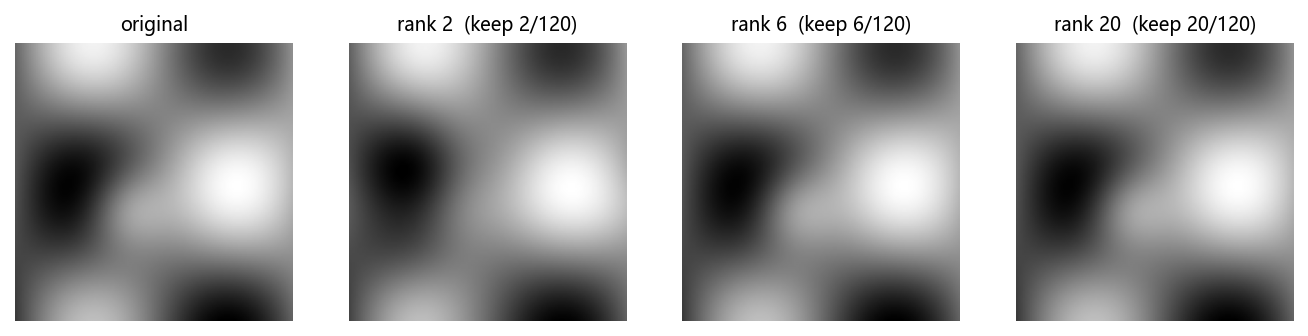
\includegraphics[keepaspectratio,alt={SVD 压缩示例}]{figures/01-numpy/svd_compression.png}}
\caption{SVD 压缩示例}
\end{figure}

\subsubsection{3.3.3 Cholesky 分解}\label{cholesky-ux5206ux89e3}

要求矩阵\textbf{对称正定}：

\begin{Shaded}
\begin{Highlighting}[]
\NormalTok{A }\OperatorTok{=}\NormalTok{ np.array([[}\FloatTok{4.}\NormalTok{, }\FloatTok{2.}\NormalTok{], [}\FloatTok{2.}\NormalTok{, }\FloatTok{3.}\NormalTok{]])}
\NormalTok{L }\OperatorTok{=}\NormalTok{ np.linalg.cholesky(A)}
\BuiltInTok{print}\NormalTok{(L)          }\CommentTok{\# [[2. 0. ][1. 1.4142]]}
\BuiltInTok{print}\NormalTok{(L }\OperatorTok{@}\NormalTok{ L.T)    }\CommentTok{\# ≈ A}
\end{Highlighting}
\end{Shaded}

\subsubsection{3.3.4 QR 分解}\label{qr-ux5206ux89e3}

\begin{Shaded}
\begin{Highlighting}[]
\NormalTok{A }\OperatorTok{=}\NormalTok{ np.array([[}\FloatTok{12.}\NormalTok{, }\OperatorTok{{-}}\FloatTok{51.}\NormalTok{], [}\FloatTok{6.}\NormalTok{, }\FloatTok{167.}\NormalTok{], [}\OperatorTok{{-}}\FloatTok{4.}\NormalTok{, }\FloatTok{24.}\NormalTok{]])}
\NormalTok{Q, R }\OperatorTok{=}\NormalTok{ np.linalg.qr(A)}
\BuiltInTok{print}\NormalTok{(Q.shape, R.shape)   }\CommentTok{\# (3,2) (2,2)}
\BuiltInTok{print}\NormalTok{(np.allclose(Q }\OperatorTok{@}\NormalTok{ R, A))   }\CommentTok{\# True}
\end{Highlighting}
\end{Shaded}

QR 在最小二乘、特征值算法稳定实现中广泛使用。

\begin{center}\rule{0.5\linewidth}{0.5pt}\end{center}

\subsection{常见误区}\label{ux5e38ux89c1ux8befux533a-2}

\begin{enumerate}
\def\labelenumi{\arabic{enumi}.}
\tightlist
\item
  \textbf{对非方阵用 \texttt{inv}}：应使用 \texttt{pinv} 或
  \texttt{lstsq}。
\item
  \textbf{认为 \texttt{eig}
  对任意矩阵都可用}：特征值分解只对方阵；非方阵用 SVD。
\item
  \textbf{忽略条件数}：\texttt{solve} 计算成功 ≠ 解可靠，先看
  \texttt{cond}。
\item
  \textbf{SVD 返回的 \texttt{S} 不是对角矩阵}：需要 \texttt{np.diag(S)}
  构造。
\item
  \textbf{\texttt{full\_matrices=False}
  与非默认的区别}：不关心零奇异值/补全正交基时，用
  \texttt{full\_matrices=False} 更省内存。
\end{enumerate}

\subsection{思考题}\label{ux601dux8003ux9898-2}

\begin{enumerate}
\def\labelenumi{\arabic{enumi}.}
\tightlist
\item
  为什么 \texttt{cond(A)} 很大时，\texttt{np.linalg.solve(A,\ b)}
  的结果可能仍``看起来正常''？
\item
  SVD 的 \texttt{U}、\texttt{Vt} 与 \texttt{eig}
  的特征向量有什么联系（提示：\texttt{A\^{}T\ A}）？
\item
  若只保留前 1 个奇异值做近似，误差如何估计？
\end{enumerate}

\subsection{动手练习（详见
lab）}\label{ux52a8ux624bux7ec3ux4e60ux8be6ux89c1-lab-2}

\begin{itemize}
\tightlist
\item
  解一个 \(4\times4\) 线性方程组 3 组（含病态）并比较解；
\item
  对 10×5 矩阵做 SVD，比较 rank 1/3/5 重构误差；
\item
  用 Cholesky 验证正定矩阵的分解唯一性。
\end{itemize}

\subsection{延伸阅读}\label{ux5ef6ux4f38ux9605ux8bfb-2}

\begin{itemize}
\tightlist
\item
  NumPy 官方 linalg
  参考：https://numpy.org/doc/stable/reference/routines.linalg.html
\item
  NumPy 官方广播与 linalg
  教程：https://numpy.org/doc/stable/reference/routines.linalg.html\#module-numpy.linalg
\item
  SciPy Lecture Notes --
  线性代数：https://scipy-lectures.org/intro/scipy.html\#linear-algebra
\end{itemize}

\section{04
多项式与拟合：poly1d、求根与最小二乘拟合}\label{ux591aux9879ux5f0fux4e0eux62dfux5408poly1dux6c42ux6839ux4e0eux6700ux5c0fux4e8cux4e58ux62dfux5408}

\begin{quote}
本节对应原版 1.4 的内容，并增补学习目标、常见误区、思考题与延伸阅读。
配套图：\texttt{figures/01-numpy/polyfit.png}。
\end{quote}

\subsection{本节目标}\label{ux672cux8282ux76eeux6807-3}

\begin{itemize}
\tightlist
\item
  会用 \texttt{np.poly1d} 构造、求值、加减乘除多项式；
\item
  会求导（\texttt{deriv}）、积分（\texttt{integ}）、求根（\texttt{np.roots}）；
\item
  会用 \texttt{np.polyfit} / \texttt{np.polyval}
  做最小二乘拟合，并理解``过拟合''现象；
\item
  知道新版 \texttt{np.polynomial.Polynomial} 的方向（便于迁移）。
\end{itemize}

\subsection{先修}\label{ux5148ux4fee-3}

\begin{itemize}
\tightlist
\item
  01 数组基础、02 数组运算；了解``多项式系数按最高次到常数排列''。
\end{itemize}

\begin{center}\rule{0.5\linewidth}{0.5pt}\end{center}

\subsection{4.1
多项式的构造与运算}\label{ux591aux9879ux5f0fux7684ux6784ux9020ux4e0eux8fd0ux7b97}

\begin{Shaded}
\begin{Highlighting}[]
\ImportTok{import}\NormalTok{ numpy }\ImportTok{as}\NormalTok{ np}

\CommentTok{\#\# 2x\^{}2 + 3x + 1}
\NormalTok{p }\OperatorTok{=}\NormalTok{ np.poly1d([}\DecValTok{2}\NormalTok{, }\DecValTok{3}\NormalTok{, }\DecValTok{1}\NormalTok{])}
\BuiltInTok{print}\NormalTok{(p)          }\CommentTok{\# 2 x\^{}2 + 3 x + 1}
\BuiltInTok{print}\NormalTok{(p(}\DecValTok{5}\NormalTok{))       }\CommentTok{\# 66}
\end{Highlighting}
\end{Shaded}

\begin{Shaded}
\begin{Highlighting}[]
\NormalTok{   2}
\NormalTok{2 x + 3 x + 1}
\NormalTok{66}
\end{Highlighting}
\end{Shaded}

\subsubsection{4.1.1 四则运算}\label{ux56dbux5219ux8fd0ux7b97}

\begin{Shaded}
\begin{Highlighting}[]
\NormalTok{p }\OperatorTok{=}\NormalTok{ np.poly1d([}\DecValTok{2}\NormalTok{, }\DecValTok{3}\NormalTok{, }\DecValTok{1}\NormalTok{])       }\CommentTok{\# 2x\^{}2+3x+1}
\NormalTok{q }\OperatorTok{=}\NormalTok{ np.poly1d([}\DecValTok{1}\NormalTok{, }\OperatorTok{{-}}\DecValTok{1}\NormalTok{])         }\CommentTok{\# x {-} 1}

\BuiltInTok{print}\NormalTok{(p }\OperatorTok{+}\NormalTok{ q)      }\CommentTok{\# 加法}
\BuiltInTok{print}\NormalTok{(p }\OperatorTok{{-}}\NormalTok{ q)      }\CommentTok{\# 减法}
\BuiltInTok{print}\NormalTok{(p }\OperatorTok{*}\NormalTok{ q)      }\CommentTok{\# 乘法（系数卷积）}
\BuiltInTok{print}\NormalTok{(p }\OperatorTok{/}\NormalTok{ q)      }\CommentTok{\# 除法 → (商, 余数) 元组}
\end{Highlighting}
\end{Shaded}

\begin{Shaded}
\begin{Highlighting}[]
\NormalTok{quotient, remainder }\OperatorTok{=}\NormalTok{ p }\OperatorTok{/}\NormalTok{ q    }\CommentTok{\# poly1d 直接除返回 (商, 余数) 元组}
\BuiltInTok{print}\NormalTok{(quotient)   }\CommentTok{\# 商}
\BuiltInTok{print}\NormalTok{(remainder)  }\CommentTok{\# 余数}

\CommentTok{\#\# 也可用 numpy.polydiv（传入系数）}
\NormalTok{q\_, r\_ }\OperatorTok{=}\NormalTok{ np.polydiv(p.coeffs, q.coeffs)}
\end{Highlighting}
\end{Shaded}

\subsubsection{4.1.2 求导与积分}\label{ux6c42ux5bfcux4e0eux79efux5206}

\begin{Shaded}
\begin{Highlighting}[]
\NormalTok{p }\OperatorTok{=}\NormalTok{ np.poly1d([}\DecValTok{2}\NormalTok{, }\DecValTok{3}\NormalTok{, }\DecValTok{1}\NormalTok{])}
\BuiltInTok{print}\NormalTok{(p.deriv())      }\CommentTok{\# 4x + 3}
\BuiltInTok{print}\NormalTok{(p.deriv(}\DecValTok{2}\NormalTok{))     }\CommentTok{\# 二阶导}
\BuiltInTok{print}\NormalTok{(p.integ())      }\CommentTok{\# 0.6667x\^{}3 + 1.5x\^{}2 + x（常数默认为 0）}
\BuiltInTok{print}\NormalTok{(p.integ(m}\OperatorTok{=}\DecValTok{2}\NormalTok{))   }\CommentTok{\# 二重积分}
\end{Highlighting}
\end{Shaded}

\subsubsection{4.1.3 系数与求根}\label{ux7cfbux6570ux4e0eux6c42ux6839}

\begin{Shaded}
\begin{Highlighting}[]
\NormalTok{p }\OperatorTok{=}\NormalTok{ np.poly1d([}\DecValTok{1}\NormalTok{, }\OperatorTok{{-}}\DecValTok{3}\NormalTok{, }\DecValTok{2}\NormalTok{])     }\CommentTok{\# x\^{}2 {-} 3x + 2}
\BuiltInTok{print}\NormalTok{(p.coeffs)               }\CommentTok{\# [ 1. {-}3.  2.]}
\BuiltInTok{print}\NormalTok{(p.c)                    }\CommentTok{\# 按降幂的系数}
\NormalTok{np.roots(p)                   }\CommentTok{\# [2. 1.]}
\end{Highlighting}
\end{Shaded}

\begin{quote}
\texttt{np.roots}
也支持直接传系数数组：\texttt{np.roots({[}1,\ -3,\ 2{]})}。
\end{quote}

\begin{center}\rule{0.5\linewidth}{0.5pt}\end{center}

\subsection{4.2
最小二乘拟合：polyfit}\label{ux6700ux5c0fux4e8cux4e58ux62dfux5408polyfit}

\begin{Shaded}
\begin{Highlighting}[]
\NormalTok{x }\OperatorTok{=}\NormalTok{ np.array([}\DecValTok{0}\NormalTok{, }\DecValTok{1}\NormalTok{, }\DecValTok{2}\NormalTok{, }\DecValTok{3}\NormalTok{, }\DecValTok{4}\NormalTok{], dtype}\OperatorTok{=}\BuiltInTok{float}\NormalTok{)}
\NormalTok{y }\OperatorTok{=}\NormalTok{ np.array([}\DecValTok{1}\NormalTok{, }\DecValTok{2}\NormalTok{, }\DecValTok{9}\NormalTok{, }\DecValTok{28}\NormalTok{, }\DecValTok{65}\NormalTok{], dtype}\OperatorTok{=}\BuiltInTok{float}\NormalTok{)   }\CommentTok{\# 恰好是 x\^{}3 + 1}

\NormalTok{coef }\OperatorTok{=}\NormalTok{ np.polyfit(x, y, }\DecValTok{3}\NormalTok{)       }\CommentTok{\# 3 次多项式最小二乘}
\BuiltInTok{print}\NormalTok{(coef)                      }\CommentTok{\# [ 1.  0. {-}0.  1.]}
\NormalTok{p }\OperatorTok{=}\NormalTok{ np.poly1d(coef)}
\BuiltInTok{print}\NormalTok{(p)                         }\CommentTok{\# 1 x\^{}3 + 0 x\^{}2 + 0 x + 1}
\BuiltInTok{print}\NormalTok{(np.polyval(coef, }\FloatTok{2.5}\NormalTok{))     }\CommentTok{\# 16.625}
\end{Highlighting}
\end{Shaded}

\textbf{含噪声数据的拟合与过拟合}：

\begin{Shaded}
\begin{Highlighting}[]
\ImportTok{import}\NormalTok{ numpy }\ImportTok{as}\NormalTok{ np}
\ImportTok{import}\NormalTok{ matplotlib.pyplot }\ImportTok{as}\NormalTok{ plt}

\NormalTok{np.random.seed(}\DecValTok{7}\NormalTok{)}
\KeywordTok{def}\NormalTok{ f(x): }\ControlFlowTok{return} \DecValTok{2} \OperatorTok{*}\NormalTok{ x }\OperatorTok{**} \DecValTok{2} \OperatorTok{{-}} \DecValTok{3} \OperatorTok{*}\NormalTok{ x }\OperatorTok{+} \DecValTok{1}
\NormalTok{x }\OperatorTok{=}\NormalTok{ np.linspace(}\OperatorTok{{-}}\DecValTok{2}\NormalTok{, }\DecValTok{3}\NormalTok{, }\DecValTok{40}\NormalTok{)}
\NormalTok{y }\OperatorTok{=}\NormalTok{ f(x) }\OperatorTok{+}\NormalTok{ np.random.normal(}\DecValTok{0}\NormalTok{, }\DecValTok{2}\NormalTok{, x.size)   }\CommentTok{\# 加噪声}

\ControlFlowTok{for}\NormalTok{ deg }\KeywordTok{in}\NormalTok{ (}\DecValTok{1}\NormalTok{, }\DecValTok{3}\NormalTok{, }\DecValTok{5}\NormalTok{):}
\NormalTok{    coef }\OperatorTok{=}\NormalTok{ np.polyfit(x, y, deg)}
    \BuiltInTok{print}\NormalTok{(deg, }\StringTok{":"}\NormalTok{, coef)}

\CommentTok{\#\# 绘图}
\NormalTok{xs }\OperatorTok{=}\NormalTok{ np.linspace(}\OperatorTok{{-}}\DecValTok{2}\NormalTok{, }\DecValTok{3}\NormalTok{, }\DecValTok{200}\NormalTok{)}
\NormalTok{plt.scatter(x, y, s}\OperatorTok{=}\DecValTok{16}\NormalTok{, label}\OperatorTok{=}\StringTok{"data"}\NormalTok{)}
\ControlFlowTok{for}\NormalTok{ deg, c, ls }\KeywordTok{in}\NormalTok{ [(}\DecValTok{1}\NormalTok{, }\StringTok{"grey"}\NormalTok{, }\StringTok{"{-}{-}"}\NormalTok{), (}\DecValTok{3}\NormalTok{, }\StringTok{"orange"}\NormalTok{, }\StringTok{"{-}."}\NormalTok{), (}\DecValTok{5}\NormalTok{, }\StringTok{"green"}\NormalTok{, }\StringTok{"{-}"}\NormalTok{)]:}
\NormalTok{    plt.plot(xs, np.polyval(np.polyfit(x, y, deg), xs), c}\OperatorTok{=}\NormalTok{c, ls}\OperatorTok{=}\NormalTok{ls, label}\OperatorTok{=}\SpecialStringTok{f"deg }\SpecialCharTok{\{}\NormalTok{deg}\SpecialCharTok{\}}\SpecialStringTok{"}\NormalTok{)}
\NormalTok{plt.legend()}\OperatorTok{;}\NormalTok{ plt.savefig(}\StringTok{"poly\_fit\_demo.png"}\NormalTok{)}
\end{Highlighting}
\end{Shaded}

\begin{figure}
\centering
\pandocbounded{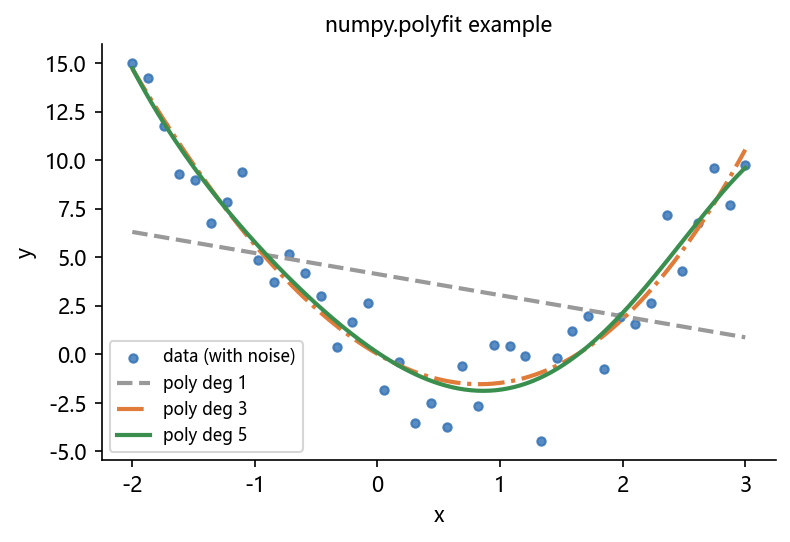
\includegraphics[keepaspectratio,alt={polyfit 示例}]{figures/01-numpy/polyfit.png}}
\caption{polyfit 示例}
\end{figure}

\textbf{观察}：次数越高，拟合曲线越可能贴近噪声（过拟合）；次数过低则拟合不足。选择次数可用交叉验证或残差分析，而不是盲目升高次数。

\begin{center}\rule{0.5\linewidth}{0.5pt}\end{center}

\subsection{4.3
新版多项式接口（了解）}\label{ux65b0ux7248ux591aux9879ux5f0fux63a5ux53e3ux4e86ux89e3}

NumPy 1.x 之后的 \texttt{np.polynomial} 提供更现代、更稳定的
\texttt{Polynomial} / \texttt{Chebyshev} 等类：

\begin{Shaded}
\begin{Highlighting}[]
\ImportTok{from}\NormalTok{ numpy.polynomial }\ImportTok{import}\NormalTok{ Polynomial}
\NormalTok{p }\OperatorTok{=}\NormalTok{ Polynomial([}\DecValTok{1}\NormalTok{, }\DecValTok{3}\NormalTok{, }\DecValTok{2}\NormalTok{])     }\CommentTok{\# 注意：系数从常数项开始！}
\BuiltInTok{print}\NormalTok{(p(}\DecValTok{2}\NormalTok{))                   }\CommentTok{\# 1 + 3*2 + 2*2\^{}2 = 15}
\BuiltInTok{print}\NormalTok{(p.roots())}
\end{Highlighting}
\end{Shaded}

\begin{quote}
\texttt{np.poly1d}
是旧接口（系数降幂、基于\texttt{np.poly}），大量教程/教材仍在使用；新代码可优先考虑
\texttt{np.polynomial}。本讲义两者都给出，以兼容常见场景。
\end{quote}

\begin{center}\rule{0.5\linewidth}{0.5pt}\end{center}

\subsection{常见误区}\label{ux5e38ux89c1ux8befux533a-3}

\begin{enumerate}
\def\labelenumi{\arabic{enumi}.}
\tightlist
\item
  \textbf{系数顺序搞反}：\texttt{poly1d({[}a,\ b,\ c{]})} 表示
  \(a x^2 + b x + c\)；\texttt{np.polynomial.Polynomial}
  则是常数项在前。
\item
  \textbf{\texttt{polyfit} 次数过高}：数据少时高次多项式会震荡/过拟合。
\item
  \textbf{忘记噪声与残差}：拟合不是``解释唯一真理''，要报告残差与预测区间。
\item
  \textbf{把 \texttt{polyfit}
  当精确解}：它是数值最小二乘，数据含噪声时系数有误差。
\end{enumerate}

\subsection{思考题}\label{ux601dux8003ux9898-3}

\begin{enumerate}
\def\labelenumi{\arabic{enumi}.}
\tightlist
\item
  \(n\) 个数据点做 \(n-1\) 次多项式拟合会出现什么现象？为什么？
\item
  \texttt{polyfit} 与 \texttt{lstsq} 的关系是什么？
\item
  如何判断``次数挑对了''？
\end{enumerate}

\subsection{动手练习（详见
lab）}\label{ux52a8ux624bux7ec3ux4e60ux8be6ux89c1-lab-3}

\begin{itemize}
\tightlist
\item
  对 \(y = 0.5x^3 - 2x + 1 + \varepsilon\) 的 30 个噪声点，分别拟合
  1/3/5 次，比较残差与测试误差；
\item
  用 \texttt{poly1d} 求 \(x^4 - 5x^2 + 4\) 的根，并验证代入为 0。
\end{itemize}

\subsection{延伸阅读}\label{ux5ef6ux4f38ux9605ux8bfb-3}

\begin{itemize}
\tightlist
\item
  NumPy 官方 polynomial
  文档：https://numpy.org/doc/stable/reference/routines.polynomials.html
\item
  NumPy 官方 polyfit
  说明：https://numpy.org/doc/stable/reference/generated/numpy.polyfit.html
\item
  SciPy Lecture Notes --
  最小二乘：https://scipy-lectures.org/intro/scipy.html\#least-squares-approximation
\end{itemize}

\section{05 综合案例：SVD
图像压缩与实验数据拟合}\label{ux7efcux5408ux6848ux4f8bsvd-ux56feux50cfux538bux7f29ux4e0eux5b9eux9a8cux6570ux636eux62dfux5408}

\begin{quote}
本章新增综合案例，用于把 01--04 的知识串起来：\textbf{形状/广播 +
线性代数 + 拟合 + 可视化}。 所有代码均可在 NumPy ≥ 1.24
环境直接运行；配图由 \texttt{build/make\_chap1\_figures.py} 生成。
\end{quote}

\subsection{案例 1：用 SVD
压缩一张``图像''}\label{ux6848ux4f8b-1ux7528-svd-ux538bux7f29ux4e00ux5f20ux56feux50cf}

\subsubsection{背景}\label{ux80ccux666f}

一张 \(m \times n\) 的灰度图可看作矩阵。SVD 给出

\[
A = U \Sigma V^T,\qquad U\in\mathbb{R}^{m\times r},\ \Sigma\in\mathbb{R}^{r\times r},\ V\in\mathbb{R}^{n\times r}
\]

只保留前 \(k\) 个奇异值，得到低秩近似

\[
A_k = U_{:,1:k}\ \Sigma_{1:k,1:k}\ V_{1:k,:}^T
\]

存储量从 \(m n\) 减少到 \(k(m+n+1)\)，当 \(k\ll \min(m,n)\) 时压缩明显。

\subsubsection{代码：生成合成图像并做低秩近似}\label{ux4ee3ux7801ux751fux6210ux5408ux6210ux56feux50cfux5e76ux505aux4f4eux79e9ux8fd1ux4f3c}

\begin{Shaded}
\begin{Highlighting}[]
\ImportTok{import}\NormalTok{ numpy }\ImportTok{as}\NormalTok{ np}
\ImportTok{import}\NormalTok{ matplotlib.pyplot }\ImportTok{as}\NormalTok{ plt}

\CommentTok{\#\# 1) 生成一张“灰度图”（120x120，含图案与明暗渐变）}
\NormalTok{x }\OperatorTok{=}\NormalTok{ np.linspace(}\DecValTok{0}\NormalTok{, }\DecValTok{1}\NormalTok{, }\DecValTok{120}\NormalTok{)}\OperatorTok{;}\NormalTok{ y }\OperatorTok{=}\NormalTok{ np.linspace(}\DecValTok{0}\NormalTok{, }\DecValTok{1}\NormalTok{, }\DecValTok{120}\NormalTok{)}
\NormalTok{X, Y }\OperatorTok{=}\NormalTok{ np.meshgrid(x, y)}
\NormalTok{img }\OperatorTok{=}\NormalTok{ (np.sin(}\DecValTok{6} \OperatorTok{*}\NormalTok{ X) }\OperatorTok{*}\NormalTok{ np.cos(}\DecValTok{6} \OperatorTok{*}\NormalTok{ Y)}
       \OperatorTok{+}\NormalTok{ np.exp(}\OperatorTok{{-}}\NormalTok{((X }\OperatorTok{{-}} \FloatTok{0.4}\NormalTok{) }\OperatorTok{**} \DecValTok{2} \OperatorTok{+}\NormalTok{ (Y }\OperatorTok{{-}} \FloatTok{0.6}\NormalTok{) }\OperatorTok{**} \DecValTok{2}\NormalTok{) }\OperatorTok{*} \DecValTok{40}\NormalTok{)}
       \OperatorTok{+} \FloatTok{0.6} \OperatorTok{*}\NormalTok{ X }\OperatorTok{{-}} \FloatTok{0.4} \OperatorTok{*}\NormalTok{ Y)}
\NormalTok{img }\OperatorTok{=}\NormalTok{ (img }\OperatorTok{{-}}\NormalTok{ img.}\BuiltInTok{min}\NormalTok{()) }\OperatorTok{/}\NormalTok{ (img.}\BuiltInTok{max}\NormalTok{() }\OperatorTok{{-}}\NormalTok{ img.}\BuiltInTok{min}\NormalTok{())}

\CommentTok{\#\# 2) SVD}
\NormalTok{U, S, Vt }\OperatorTok{=}\NormalTok{ np.linalg.svd(img, full\_matrices}\OperatorTok{=}\VariableTok{False}\NormalTok{)}

\CommentTok{\#\# 3) 不同秩的重建与误差}
\ControlFlowTok{for}\NormalTok{ k }\KeywordTok{in}\NormalTok{ (}\DecValTok{2}\NormalTok{, }\DecValTok{6}\NormalTok{, }\DecValTok{20}\NormalTok{):}
\NormalTok{    A\_k }\OperatorTok{=}\NormalTok{ U[:, :k] }\OperatorTok{@}\NormalTok{ np.diag(S[:k]) }\OperatorTok{@}\NormalTok{ Vt[:k, :]}
\NormalTok{    mse }\OperatorTok{=}\NormalTok{ np.mean((img }\OperatorTok{{-}}\NormalTok{ A\_k) }\OperatorTok{**} \DecValTok{2}\NormalTok{)}
\NormalTok{    params }\OperatorTok{=}\NormalTok{ k }\OperatorTok{*}\NormalTok{ (img.shape[}\DecValTok{0}\NormalTok{] }\OperatorTok{+} \DecValTok{1} \OperatorTok{+}\NormalTok{ img.shape[}\DecValTok{1}\NormalTok{])}
    \BuiltInTok{print}\NormalTok{(}\SpecialStringTok{f"rank=}\SpecialCharTok{\{}\NormalTok{k}\SpecialCharTok{:2d\}}\SpecialStringTok{  MSE=}\SpecialCharTok{\{}\NormalTok{mse}\SpecialCharTok{:.5f\}}\SpecialStringTok{  存储量=}\SpecialCharTok{\{}\NormalTok{params}\SpecialCharTok{\}}\SpecialStringTok{ / 原图=}\SpecialCharTok{\{}\NormalTok{img}\SpecialCharTok{.}\NormalTok{size}\SpecialCharTok{\}}\SpecialStringTok{ "}
          \SpecialStringTok{f"(}\SpecialCharTok{\{}\DecValTok{100}\OperatorTok{*}\NormalTok{params}\OperatorTok{/}\NormalTok{img}\SpecialCharTok{.}\NormalTok{size}\SpecialCharTok{:.1f\}}\SpecialStringTok{\%)"}\NormalTok{)}
\end{Highlighting}
\end{Shaded}

\begin{Shaded}
\begin{Highlighting}[]
\NormalTok{rank= 2  MSE=0.00087  存储量=482 / 原图=14400 (3.3\%)}
\NormalTok{rank= 6  MSE=0.00000  存储量=1446 / 原图=14400 (10.0\%)}
\NormalTok{rank=20  MSE=0.00000  存储量=4820 / 原图=14400 (33.5\%)}
\end{Highlighting}
\end{Shaded}

\begin{figure}
\centering
\pandocbounded{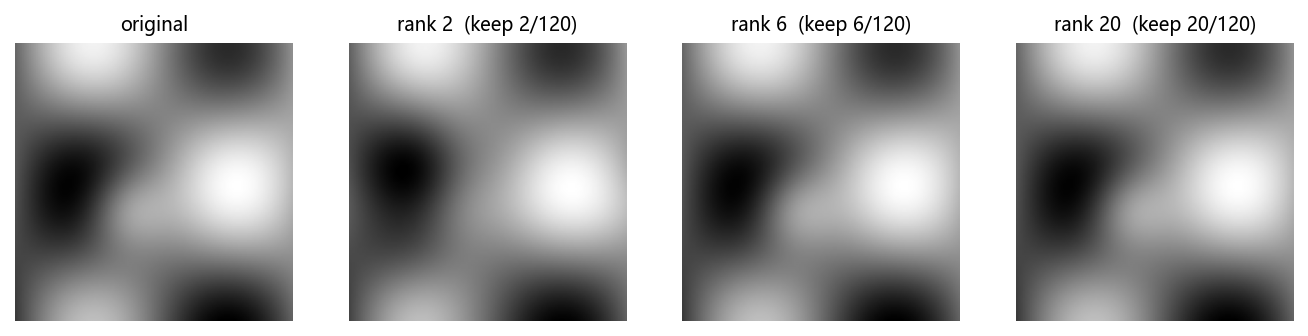
\includegraphics[keepaspectratio,alt={SVD 图像压缩}]{figures/01-numpy/svd_compression.png}}
\caption{SVD 图像压缩}
\end{figure}

\subsubsection{分析}\label{ux5206ux6790}

\begin{itemize}
\tightlist
\item
  rank=2 时仅用 3.3\% 的存储量，MSE≈0.0009（肉眼几乎无差别）；
\item
  rank=6 之后误差已低于打印精度；
\item
  说明\textbf{自然图像的能量高度集中在前几个奇异值}------这正是图像压缩、PCA、数据降维的共同原理。
\end{itemize}

\subsubsection{拓展任务}\label{ux62d3ux5c55ux4efbux52a1}

\begin{enumerate}
\def\labelenumi{\arabic{enumi}.}
\tightlist
\item
  用
  \texttt{np.linalg.norm(img\ -\ A\_k,\ \textquotesingle{}fro\textquotesingle{})}
  计算相对误差；
\item
  对一张真实图片（PIL 读取灰度化）重复实验，观察``压缩率 vs 视觉质量'';
\item
  把 \texttt{img} 换成随机噪声图，观察奇异值衰减是否还那么快？为什么？
\end{enumerate}

\begin{center}\rule{0.5\linewidth}{0.5pt}\end{center}

\subsection{案例
2：实验数据的最小二乘拟合}\label{ux6848ux4f8b-2ux5b9eux9a8cux6570ux636eux7684ux6700ux5c0fux4e8cux4e58ux62dfux5408}

\subsubsection{背景}\label{ux80ccux666f-1}

物理实验得到一组 \((x_i, y_i)\)，理论公式是二次函数，但测量有噪声。用
\texttt{np.polyfit} 求 \(y = a x^2 + b x + c\)
的最佳系数，并评估拟合质量。

\subsubsection{代码}\label{ux4ee3ux7801}

\begin{Shaded}
\begin{Highlighting}[]
\ImportTok{import}\NormalTok{ numpy }\ImportTok{as}\NormalTok{ np}
\ImportTok{import}\NormalTok{ matplotlib.pyplot }\ImportTok{as}\NormalTok{ plt}

\NormalTok{np.random.seed(}\DecValTok{7}\NormalTok{)}
\KeywordTok{def}\NormalTok{ theory(x): }\ControlFlowTok{return} \DecValTok{2} \OperatorTok{*}\NormalTok{ x }\OperatorTok{**} \DecValTok{2} \OperatorTok{{-}} \DecValTok{3} \OperatorTok{*}\NormalTok{ x }\OperatorTok{+} \DecValTok{1}

\NormalTok{x }\OperatorTok{=}\NormalTok{ np.linspace(}\OperatorTok{{-}}\DecValTok{2}\NormalTok{, }\DecValTok{3}\NormalTok{, }\DecValTok{40}\NormalTok{)}
\NormalTok{y }\OperatorTok{=}\NormalTok{ theory(x) }\OperatorTok{+}\NormalTok{ np.random.normal(}\DecValTok{0}\NormalTok{, }\DecValTok{2}\NormalTok{, x.size)   }\CommentTok{\# 加噪声}

\NormalTok{coef2 }\OperatorTok{=}\NormalTok{ np.polyfit(x, y, }\DecValTok{2}\NormalTok{)      }\CommentTok{\# 二次拟合}
\NormalTok{coef5 }\OperatorTok{=}\NormalTok{ np.polyfit(x, y, }\DecValTok{5}\NormalTok{)      }\CommentTok{\# 五次拟合（对比）}
\BuiltInTok{print}\NormalTok{(}\StringTok{"二次系数 (a,b,c):"}\NormalTok{, np.}\BuiltInTok{round}\NormalTok{(coef2, }\DecValTok{3}\NormalTok{))}
\BuiltInTok{print}\NormalTok{(}\StringTok{"五次系数:"}\NormalTok{, np.}\BuiltInTok{round}\NormalTok{(coef5, }\DecValTok{3}\NormalTok{))}

\CommentTok{\#\# 残差（RMSE）}
\NormalTok{rmse2 }\OperatorTok{=}\NormalTok{ np.sqrt(np.mean((np.polyval(coef2, x) }\OperatorTok{{-}}\NormalTok{ y) }\OperatorTok{**} \DecValTok{2}\NormalTok{))}
\NormalTok{rmse5 }\OperatorTok{=}\NormalTok{ np.sqrt(np.mean((np.polyval(coef5, x) }\OperatorTok{{-}}\NormalTok{ y) }\OperatorTok{**} \DecValTok{2}\NormalTok{))}
\BuiltInTok{print}\NormalTok{(}\SpecialStringTok{f"RMSE(deg2)=}\SpecialCharTok{\{}\NormalTok{rmse2}\SpecialCharTok{:.3f\}}\SpecialStringTok{  RMSE(deg5)=}\SpecialCharTok{\{}\NormalTok{rmse5}\SpecialCharTok{:.3f\}}\SpecialStringTok{"}\NormalTok{)}
\end{Highlighting}
\end{Shaded}

\begin{Shaded}
\begin{Highlighting}[]
\NormalTok{二次系数 (a,b,c): [ 2.123 {-}3.231  0.616]}
\NormalTok{五次系数: [{-}0.010  0.210 {-}0.278  1.206 {-}2.469  1.162]}
\NormalTok{RMSE(deg2)=2.116  RMSE(deg5)=2.026}
\end{Highlighting}
\end{Shaded}

\subsubsection{分析}\label{ux5206ux6790-1}

\begin{itemize}
\tightlist
\item
  二次拟合系数接近真实值
  \((2, -3, 1)\)，说明模型设定正确时最小二乘能恢复参数；
\item
  五次拟合在训练数据上的 RMSE 略低（2.026 vs
  2.116），说明``次数越高越能贴合训练数据''------但这是\textbf{过拟合的征兆}；
\item
  把前 28 个点作训练、后 12
  个点作\textbf{独立测试}时：\texttt{deg2\ 测试\ RMSE≈3.11}，而
  \texttt{deg5\ 测试\ RMSE≈139.1}！过拟合在测试集上暴露无遗。因此选次数必须看独立测试集/交叉验证，而不是训练误差。
\end{itemize}

\begin{figure}
\centering
\pandocbounded{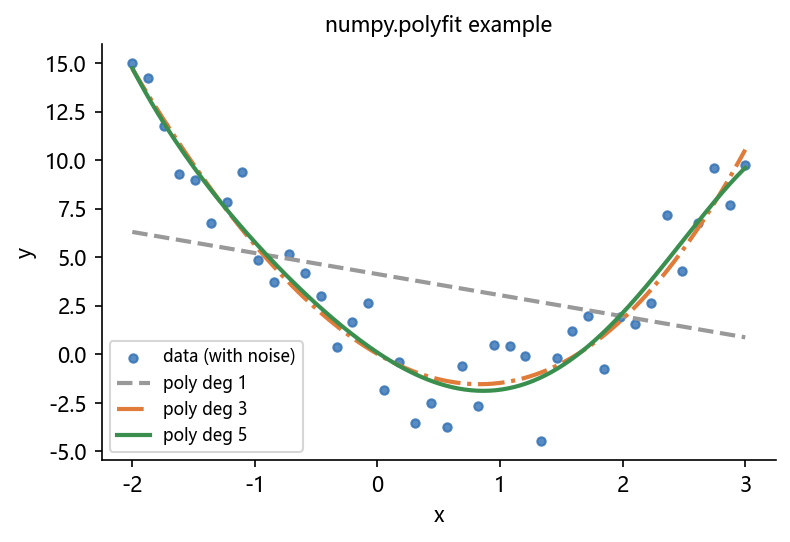
\includegraphics[keepaspectratio,alt={polyfit 示例}]{figures/01-numpy/polyfit.png}}
\caption{polyfit 示例}
\end{figure}

\subsubsection{拓展任务}\label{ux62d3ux5c55ux4efbux52a1-1}

\begin{enumerate}
\def\labelenumi{\arabic{enumi}.}
\tightlist
\item
  划分训练/测试集（如 70/30），比较 deg=2 与 deg=5 在测试集上的
  RMSE（本案例中 deg2≈3.11，deg5≈139.1）；
\item
  用 \texttt{np.linalg.lstsq} 重写拟合，体会与 \texttt{polyfit} 的关系；
\item
  打印 95\% 置信区间（提示：用 \texttt{np.polyfit} 的 cov 参数或
  scipy.stats）。
\end{enumerate}

\begin{center}\rule{0.5\linewidth}{0.5pt}\end{center}

\subsection{本章综合练习（上机任务）}\label{ux672cux7ae0ux7efcux5408ux7ec3ux4e60ux4e0aux673aux4efbux52a1}

\begin{enumerate}
\def\labelenumi{\arabic{enumi}.}
\tightlist
\item
  生成 50×50 的``数字 + 渐变''图案，用 rank = 1, 3, 5, 10 重构并绘制 2×2
  对比图；
\item
  构造 \(y = 3e^{-x} + 2 + \varepsilon\)
  的噪声数据，尝试多项式拟合（哪种次数更合理？），并给出误差曲线；
\item
  把案例 1 与案例 2 整理成一个 \texttt{.ipynb}，写一份 200
  字以内的结论。
\end{enumerate}

\subsection{延伸阅读}\label{ux5ef6ux4f38ux9605ux8bfb-4}

\begin{itemize}
\tightlist
\item
  NumPy 官方
  SVD：https://numpy.org/doc/stable/reference/generated/numpy.linalg.svd.html
\item
  SciPy
  相关低秩近似（scipy.sparse.linalg）：https://docs.scipy.org/doc/scipy/reference/sparse.linalg.html
\item
  scikit-learn PCA
  官方示例（下一章会用到）：https://scikit-learn.org/stable/auto\_examples/index.html\#decomposition
\end{itemize}

\section{06
常见误区与技巧}\label{ux5e38ux89c1ux8befux533aux4e0eux6280ux5de7}

\begin{quote}
本章为新增``查漏补缺''页：把学生最容易踩的坑集中列出，并给出正确的写法和性能技巧。
\end{quote}

\subsection{1.
高频误区速查表}\label{ux9ad8ux9891ux8befux533aux901fux67e5ux8868}

{\def\LTcaptype{none} % do not increment counter
\begin{longtable}[]{@{}
  >{\raggedright\arraybackslash}p{(\linewidth - 6\tabcolsep) * \real{0.2500}}
  >{\raggedright\arraybackslash}p{(\linewidth - 6\tabcolsep) * \real{0.2500}}
  >{\raggedright\arraybackslash}p{(\linewidth - 6\tabcolsep) * \real{0.2500}}
  >{\raggedright\arraybackslash}p{(\linewidth - 6\tabcolsep) * \real{0.2500}}@{}}
\toprule\noalign{}
\begin{minipage}[b]{\linewidth}\raggedright
\#
\end{minipage} & \begin{minipage}[b]{\linewidth}\raggedright
误区 / 错误写法
\end{minipage} & \begin{minipage}[b]{\linewidth}\raggedright
正确做法
\end{minipage} & \begin{minipage}[b]{\linewidth}\raggedright
原因
\end{minipage} \\
\midrule\noalign{}
\endhead
\bottomrule\noalign{}
\endlastfoot
1 & \texttt{A\ *\ B} 当矩阵乘法 & \texttt{A\ @\ B} 或
\texttt{np.matmul(A,\ B)} & \texttt{*} 是逐元素乘（ufunc） \\
2 & \texttt{np.zeros(2,\ 3)} & \texttt{np.zeros((2,\ 3))} &
形状要传元组，两个括号 \\
3 & 以为 \texttt{reshape} 是拷贝 & 需要独立数据用
\texttt{arr.reshape(...).copy()} & 连续内存的 reshape 是视图 \\
4 & \texttt{x{[}x\ \textgreater{}\ 0\ and\ x\ \textless{}\ 5{]}} &
\texttt{x{[}(x\ \textgreater{}\ 0)\ \&\ (x\ \textless{}\ 5){]}} &
数组布尔运算用 \texttt{\&}，且加括号 \\
5 & \texttt{len(a)} 猜数组维数 & \texttt{a.shape}、\texttt{a.ndim} &
\texttt{len} 只给第一维长度 \\
6 & 对非方阵 \texttt{np.linalg.inv} & \texttt{np.linalg.pinv} /
\texttt{lstsq} & 逆只定义于方阵 \\
7 & \texttt{np.linalg.svd(M)} 直接 \texttt{U@S@Vt} &
\texttt{U\ @\ np.diag(S)\ @\ Vt} & \texttt{S}
是奇异值向量，不是对角阵 \\
8 & 认为 \texttt{eig} 适用于任意矩阵 & 方阵用 \texttt{eig}，任意矩阵用
\texttt{svd} & \texttt{eig} 数学条件限制 \\
9 & \texttt{np.random.rand} 不设种子 &
\texttt{rng\ =\ np.random.default\_rng(42)} & 结果不可复现 \\
10 & 循环里 \texttt{np.append} & 预分配数组或列表收集 & 每次 append
都会新建数组 \\
11 & 混淆 \texttt{axis=0/1} & 记``消除哪一维就写哪一维'' &
\texttt{sum(axis=0)} 消行得列统计 \\
12 & 用 \texttt{astype} 想``改原数组'' & \texttt{arr.astype}
返回新数组；原地改 dtype 不可直接 & 类型转换是拷贝 \\
\end{longtable}
}

\subsection{2. 原理级难点：视图 vs
拷贝}\label{ux539fux7406ux7ea7ux96beux70b9ux89c6ux56fe-vs-ux62f7ux8d1d}

\begin{Shaded}
\begin{Highlighting}[]
\NormalTok{a }\OperatorTok{=}\NormalTok{ np.arange(}\DecValTok{6}\NormalTok{)}
\NormalTok{b }\OperatorTok{=}\NormalTok{ a.reshape(}\DecValTok{2}\NormalTok{, }\DecValTok{3}\NormalTok{)     }\CommentTok{\# 视图}
\NormalTok{b[}\DecValTok{0}\NormalTok{, }\DecValTok{0}\NormalTok{] }\OperatorTok{=} \DecValTok{99}
\BuiltInTok{print}\NormalTok{(a[}\DecValTok{0}\NormalTok{])             }\CommentTok{\# 99}

\NormalTok{c }\OperatorTok{=}\NormalTok{ a.copy()}
\NormalTok{c[}\DecValTok{0}\NormalTok{] }\OperatorTok{=} \DecValTok{0}                \CommentTok{\# 不影响 a}
\end{Highlighting}
\end{Shaded}

判断是否共享内存：

\begin{Shaded}
\begin{Highlighting}[]
\NormalTok{b.base }\KeywordTok{is}\NormalTok{ a              }\CommentTok{\# True → 视图}
\NormalTok{np.may\_share\_memory(a, b)  }\CommentTok{\# 更稳的检查}
\end{Highlighting}
\end{Shaded}

\textbf{为什么重要}：视图省内存、速度快；但并发修改或函数返回到别人手里时容易``隐形改数据''。对外返回数据前，若不想共享，显式
\texttt{.copy()}。

\subsection{3. 广播规则速记}\label{ux5e7fux64adux89c4ux5219ux901fux8bb0}

\begin{enumerate}
\def\labelenumi{\arabic{enumi}.}
\tightlist
\item
  从右往左对齐；
\item
  相同或一方为 1 → 兼容；
\item
  全部兼容 → 结果为各维最大；否则 \texttt{ValueError}。
\end{enumerate}

\begin{Shaded}
\begin{Highlighting}[]
\NormalTok{A }\OperatorTok{=}\NormalTok{ np.zeros((}\DecValTok{4}\NormalTok{, }\DecValTok{1}\NormalTok{, }\DecValTok{6}\NormalTok{))}
\NormalTok{B }\OperatorTok{=}\NormalTok{ np.zeros((}\DecValTok{3}\NormalTok{, }\DecValTok{6}\NormalTok{))}
\ControlFlowTok{try}\NormalTok{:}
    \BuiltInTok{print}\NormalTok{((A }\OperatorTok{+}\NormalTok{ B).shape)     }\CommentTok{\# (4, 3, 6)，B 自动补成 (1,3,6)}
\ControlFlowTok{except} \PreprocessorTok{ValueError} \ImportTok{as}\NormalTok{ e:}
    \BuiltInTok{print}\NormalTok{(}\StringTok{"广播失败："}\NormalTok{, e)}
\end{Highlighting}
\end{Shaded}

\begin{quote}
注意：\texttt{(3,)\ +\ (4,)} 不兼容；\texttt{(3,1)\ +\ (3,)}
也不兼容（末尾 1 vs 3）。想``列向量与行向量做外积''要用
\texttt{(3,1)\ +\ (1,3)}。
\end{quote}

\subsection{4. 性能技巧}\label{ux6027ux80fdux6280ux5de7}

\begin{itemize}
\item
  \textbf{向量化优先}：能一次
  \texttt{a{[}np.newaxis,\ :{]}\ +\ b{[}:,\ np.newaxis{]}}
  就不要双重循环；
\item
  \textbf{\texttt{out=} 原地计算}：\texttt{np.add(a,\ b,\ out=a)}
  避免额外分配；
\item
  \textbf{\texttt{in-place} 算术}：\texttt{a\ +=\ b}（注意类型安全）；
\item
  \textbf{\texttt{einsum}
  表达张量收缩}：\texttt{np.einsum(\textquotesingle{}ik,kj-\textgreater{}ij\textquotesingle{},\ A,\ B)}
  既是矩阵乘，也能表达更复杂收缩且减少中间数组；
\item
  \textbf{\texttt{np.lib.stride\_tricks.sliding\_window\_view}}
  做滑窗（移动平均/卷积）时避免显式复制：

\begin{Shaded}
\begin{Highlighting}[]
\NormalTok{x }\OperatorTok{=}\NormalTok{ np.arange(}\DecValTok{10}\NormalTok{)}
\NormalTok{w }\OperatorTok{=}\NormalTok{ np.lib.stride\_tricks.sliding\_window\_view(x, }\DecValTok{3}\NormalTok{)}
\BuiltInTok{print}\NormalTok{(w.mean(axis}\OperatorTok{=}\DecValTok{1}\NormalTok{))   }\CommentTok{\# 窗口大小为 3 的移动平均}
\end{Highlighting}
\end{Shaded}
\item
  \textbf{大数组用 \texttt{np.savez\_compressed}} 存储；文本
  \texttt{savetxt} 慢且丢精度。
\end{itemize}

\subsection{5. 调试建议}\label{ux8c03ux8bd5ux5efaux8bae}

\begin{enumerate}
\def\labelenumi{\arabic{enumi}.}
\tightlist
\item
  出错先打印 \texttt{shape} / \texttt{dtype}，再用 \texttt{np.allclose}
  比较；
\item
  用 \texttt{np.set\_printoptions(precision=4,\ suppress=True)}
  让输出可读；
\item
  复杂布尔条件拆成中间变量（\texttt{mask1\ =\ ...;\ mask2\ =\ ...}）；
\item
  随机/拟合问题\textbf{固定种子}，便于复现与讨论；
\item
  用 \texttt{np.isnan} / \texttt{np.isinf} 检查异常值。
\end{enumerate}

\subsection{6.
本章小结（自测）}\label{ux672cux7ae0ux5c0fux7ed3ux81eaux6d4b}

\begin{itemize}
\tightlist
\item[$\square$]
  能解释 \texttt{dtype} 与 \texttt{itemsize}；
\item[$\square$]
  能说出 \texttt{view} vs \texttt{copy} 的 4 种情形；
\item[$\square$]
  能判断 \texttt{(2,3)+(3,)}、\texttt{(4,1)+(1,3)} 的可广播性；
\item[$\square$]
  能区分 \texttt{*}、\texttt{@}、\texttt{np.dot}；
\item[$\square$]
  能用 \texttt{solve} / \texttt{lstsq} 解不同形态方程组；
\item[$\square$]
  能用 \texttt{svd} / \texttt{polyfit} 完成 05 综合案例。
\end{itemize}

\subsection{延伸阅读}\label{ux5ef6ux4f38ux9605ux8bfb-5}

\begin{itemize}
\tightlist
\item
  NumPy 官方``NumPy for MATLAB
  users''：https://numpy.org/doc/stable/user/numpy-for-matlab-users.html
\item
  NumPy 性能建议：https://numpy.org/doc/stable/user/performance.html
\end{itemize}

\newpage
